\documentclass[fleqn]{article}
\usepackage{graphicx} 
\usepackage{here}    
\usepackage{amsmath}
\textwidth=15.0cm
\textheight=22.0cm
\topmargin=-1cm
\oddsidemargin=-0.3cm
\evensidemargin=-0.3cm


%packages
\usepackage{amsmath}
\usepackage{cite}
\usepackage[toc,page]{appendix}
\usepackage{fancyvrb}
\usepackage{tikz}
\usepackage{multicol}
\usepackage{framed}
\usepackage{pgfplots}
\usepackage{fixltx2e}
\usepackage{subfigure}
\usepackage{lscape}
\usepackage{enumitem}
\usepackage{multirow}
\usepackage{color}
\usepackage{xcolor}
\usepackage{comment}
\usepackage{changes}
\renewcommand*\descriptionlabel[1]{\hspace\leftmargin$#1$}

%tikz labraries
\usetikzlibrary{matrix}
\usetikzlibrary{decorations.pathreplacing}
\usetikzlibrary{positioning}
\usetikzlibrary{calc}
\usetikzlibrary{shapes,arrows, chains}
\usetikzlibrary{intersections}
\usetikzlibrary{decorations.markings}
\usetikzlibrary{calc,intersections}
\usetikzlibrary{patterns}


\makeatletter
\def\mathcolor#1#{\@mathcolor{#1}}
\def\@mathcolor#1#2#3{%
  \protect\leavevmode
  \begingroup
    \color#1{#2}#3%
  \endgroup
}
\makeatother

%##### DEFINE YOUR NAME #########################
\definechangesauthor[color=blue,name={Arpad Rozsas}]{AR}
\definechangesauthor[color=red,name={Nadieh Meinen}]{NEM}
%###########################################

\begin{document}



\pagebreak


%\documentclass[fleqn]{article}
%\usepackage{graphicx} 
%\usepackage{here}    
%\usepackage{amsmath}
%\textwidth=15.0cm
%\textheight=22.0cm
%\topmargin=-1cm
%\oddsidemargin=-0.3cm
%\evensidemargin=-0.3cm
%
%
%%packages
%\usepackage{amsmath}
%\usepackage{cite}
%\usepackage[toc,page]{appendix}
%\usepackage{fancyvrb}
%\usepackage{tikz}
%\usepackage{multicol}
%\usepackage{framed}
%\usepackage{pgfplots}
%\usepackage{fixltx2e}
%\usepackage{subfigure}
%\usepackage{lscape}
%\usepackage{enumitem}
%\usepackage{multirow}
%\usepackage{color}
%\usepackage{xcolor}
%\usepackage{comment}
%\usepackage{changes}
%\renewcommand*\descriptionlabel[1]{\hspace\leftmargin$#1$}
%
%%tikz labraries
%\usetikzlibrary{matrix}
%\usetikzlibrary{decorations.pathreplacing}
%\usetikzlibrary{positioning}
%\usetikzlibrary{calc}
%\usetikzlibrary{shapes,arrows, chains}
%\usetikzlibrary{intersections}
%\usetikzlibrary{decorations.markings}
%\usetikzlibrary{calc,intersections}
%\usetikzlibrary{patterns}
%
%
%\makeatletter
%\def\mathcolor#1#{\@mathcolor{#1}}
%\def\@mathcolor#1#2#3{%
%  \protect\leavevmode
%  \begingroup
%    \color#1{#2}#3%
%  \endgroup
%}
%\makeatother
%
%%##### DEFINE YOUR NAME #########################
%\definechangesauthor[color=blue,name={Arpad Rozsas}]{AR}
%\definechangesauthor[color=red,name={Nadieh Meinen}]{NEM}
%%###########################################
%
%\begin{document}


\title{Reliability-based importance assessment of the components in the probabilistic wind load model for static structural members}
\maketitle


%\begin{framed}
%This paper investigates the effects of modeling choices in the probabilistic modeling of each of the elements in the probabilistic wind load model. The effects are assessed through the probaiblistic modeling of a generic steel element. The effects of statistical and sampling uncertainties in the wind speeds and the pressure coefficients are investigated. The effects of wind directionality
%\end{framed}

\begin{abstract}
\added[id=NEM]{Abstract, to be added}
%Wind is the governing environmental action for many structures and structural members.
%
%Especially structural members subject to local wind loads, such as facade or roof elements are vulnerable with respect to wind loading \cite{Geurts_2004}. 
%
%To derive minimum design loads to be prescribed by standards reliability analysis needs to be conducted. 
%
%
%
%
%
% Therefore, appropriate structural design of these wind-loaded members is of great importance. 
%To obtain appropriate semi-probabilistic design formats for wind loads to be used in practice, 
%a proper determination of the structural reliability of these members is of great importance in engineering. 
%
%On the basis of appropriate modeling lays structural reliability analysis, from which, when needed semi-probabilistic design formats can be derived. 
%
%The calculation of the structural reliability of these members requires appropriate physical and probabilistic modeling of both the wind loads and the structural resistance. 
%
%For the physical modeling of the wind loads the Davenport Wind Loading Chain is widely accepted. Despite the advances in wind engineering, the probabilistic description of each of the links in the chain is still under active debates, i.e. a lot of modeling choices. 
% 
%The primary objective of this paper is to investigate the effects of these modeling choices in terms of the (differences in) obtained structural reliability. Focus lies on dynamically insensitive structural members, of which local wind loads are of imporance only.  
%
%For this, we adopt a comprehensive (case-study-based) approach where all relevant components are represented as probabilistic models. The influence of modeling choices is assessed through the reliability of a generic structural member. This in contrast to the typical approach, which concentrates on the in-depth probabilistic analysis of a selected link in the chain only. 
%
%We will look for the influence of:
%* influence of taking into account wind-directionality
%  - influence of correlation between adjacent failure probabilities
%  - influence of building orientation
%* the influence of adopted distribution types
%* the influence of sampling uncertainties 
%* the influence of modeling roughness factor
%* the influence of modeling uncertainties.. 
%
%When available, the probabilistic models are established using measurements, otherwise use is made of relevant literature. The probabilistic resistance model of the structural member is varied to cover a wide range of failure modes and design formats. 
%
%The results show that... something like:
%* It is / is not relevant to take into account wind directionality effects 
%* It is / is not relevant to take into account different dist. types
%* Is is / is not relevant to take into account statistical uncertainties 
%* influence of modeling terrain effects negleglible in case of using proper values
%* Influence of modeling structural reliability is / is not negleglible on end-result beta (codification...)
%
%
\end{abstract}



\begin{centering}
\vspace{0.2cm}
Meinen N.E.\textsuperscript{a},  R\' ozs\'as A.\textsuperscript{a}, Steenbergen R.D.J.M.\textsuperscript{ab}\\
\vspace{0.2cm}
\textsuperscript{a} Department of Structural Reliability, TNO, Delft, The Netherlands\\
\textsuperscript{b} Department of Structural Engineering, Ghent University, Belgium\\
\vspace{0.2cm}
\textbf{Keywords}: wind engineering, structural reliability, probabilistic wind load model, wind-directionality, structural components
\end{centering}

%\end{document}
\documentclass[fleqn]{article}
\usepackage{graphicx} 
\usepackage{here}    
\usepackage{amsmath}
\textwidth=15.0cm
\textheight=22.0cm
\topmargin=-1cm
\oddsidemargin=-0.3cm
\evensidemargin=-0.3cm


%packages
\usepackage{amsmath}
%\usepackage{cite}
\usepackage[toc,page]{appendix}
\usepackage{fancyvrb}
\usepackage{tikz}
\usepackage{multicol}
\usepackage{framed}
\usepackage{pgfplots}
\usepackage{fixltx2e}
\usepackage{subfigure}
\usepackage{lscape}
\usepackage{enumitem}
\usepackage{multirow}
\usepackage{color}
\usepackage{xcolor}
\usepackage{comment}
\usepackage{changes}
\renewcommand*\descriptionlabel[1]{\hspace\leftmargin$#1$}

%tikz labraries
\usetikzlibrary{matrix}
\usetikzlibrary{decorations.pathreplacing}
\usetikzlibrary{positioning}
\usetikzlibrary{calc}
\usetikzlibrary{shapes,arrows, chains}
\usetikzlibrary{intersections}
\usetikzlibrary{decorations.markings}
\usetikzlibrary{calc,intersections}
\usetikzlibrary{patterns}


\makeatletter
\def\mathcolor#1#{\@mathcolor{#1}}
\def\@mathcolor#1#2#3{%
  \protect\leavevmode
  \begingroup
    \color#1{#2}#3%
  \endgroup
}
\makeatother

%##### DEFINE YOUR NAME #########################
\definechangesauthor[color=blue,name={Arpad Rozsas}]{AR}
\definechangesauthor[color=red,name={Nadieh Meinen}]{NEM}
%###########################################

\begin{document}

% -----------------------------------------------------------------------------------------------
% -----------------------------------------------------------------------------------------------
\section{Introduction}

% -----------------------------------------------------------------------------------------------
\subsection{Motivation}

Wind is the governing environmental action for many structures; particularly for structural members which can be especially vulnerable to wind loading [ref]. In practice, these structural members are designed using semi-probabilistic design methods, such as partial factor design, or load resistance factor design. To guarantee a safe design these semi-probabilistic methods are (should be) calibrated to codified target reliability levels. For this reliability-based calibration physical models and probabilistic models are needed. The former captures the underlying physical phenomena while the latter accounts for the associated uncertainties. In respect of structural members subject to wind, the probabilistic model of the wind load typically dominates the reliability; therefore, its correct modeling is of crucial importance. The widely accepted and applied Davenport wind load chain (DWLC) is considered here as the starting point of our investigation. The probabilistic description of uncertainties in this wind load chain is still under active debate despite the numerous advances in wind engineering [ref]. For instance, the decision on which distribution type to be used for wind extremes can lead to an order of magnitude difference in calculated failure probabilities [ref]. Other decisions and modeling choices can have similar bearing on the calculated failure probability. Therefore, it is of great importance to explore these decisions and associated uncertainties. Furthermore, some aspects, such as the effect of wind directionality and handling of statistical uncertainties, are not yet sufficiently explored. These issues are of particular interest for standardization committees which have few, well-reasoned guidance on probabilistic wind load models. Hence, the aim of this paper is to investigate the effect of some modeling choices and prevalently overlooked aspects using a comprehensive framework by assessing their practical, engineering relevance.

% -----------------------------------------------------------------------------------------------
\subsection{Problem statement}

The typical approach in investigating the influence of modeling choices in the probabilistic wind load chain (DWLC) concentrates on the in-depth analysis of selected links in the chain. Due to this isolated treatment the modeling choices are often compared on the basis of measures with low to moderate engineering relevance, e.g. using statistical goodness-of-fit measures [ref] or comparing representative fractiles [ref]. Given that design methods should ensure a minimum target reliability level we adopt structural reliability as a measure with high practical relevance to evaluate modeling choices. This entails that all relevant parameters in the structural reliability problem be represented with probabilistic models, e.g. modeled as random variables. Although there are studies that consider all relevant parameters with probabilistic models they lack the comparison of alternative modeling choices []. Furthermore, certain aspects of the wind load chain have received less research attention, for example the effect of wind directionality and statistical uncertainties due to data scarcity are often neglected [ref]. A more detailed overview of previous works is given in Section \ref{sec:review}.

The shortcomings of previous studies can be categorized as: (\textit{i}) not all links in the wind load chain are represented with probabilistic models; (\textit{ii}) alternative modeling choices are not compared; (\textit{iii}) measures with low or moderate engineering relevance are used to compare the modeling choices.
This paper attempts to address these shortcomings; however, it is acknowledged that such broad questions cannot be thoroughly covered and answered in a single paper. Our main contributions are (\textit{i}) the proposal of a framework (with accompanied computer code) that represent all relevant parameters as random variables; and (\textit{ii}) the comparison of selected modeling choices, e.g. distribution type, wind directionality, and statistical uncertainties, on structural reliability. Accordingly the primary research questions of this paper are formulated as:

\textit{What is the effect of probabilistic modeling decisions in the Davenport wind load chain, such as wind directionality and statistical uncertainties, on the reliability of structural members? Which components and decisions are the most important ones?}

%Emphasize that we do not really contribute to the debate which one is to be used we just show the complete analysis and the impact on structural reliability. Identify the components which should be further investigated.

As side product of answering the primary questions one can answer some secondary questions as well. These are more relevant for practitioners and standardization committees:

\textit{What is the reliability level of wind loaded structural members designed according to Eurocodes? Are the current methods ensuring the target reliability level?}

 
 % -----------------------------------------------------------------------------------------------
\subsection{Adopted approach and contributions}

To investigate the effect of the modeling choices on structural reliability of structural members a case study is set up which serves as the main vehicle of illustration throughout this study. It is a fictitious high rise building located in Schiphol, the Netherlands. Multiple locations on the facade are considered for the structural member to explore the effect of different pressure zones. The structural member is generic which can be tuned by a couple of parameters, e.g. coefficient of variation of the resistance and associated partial factor, to represent a wide range of design situations. We surmise that the case study is sufficiently flexible and generic to allow fairly general conclusions. To have a realistic design the structural member is designed according to the general recommendations of the Eurocode. Other international standards, such as ASCE-7, AISC, [ETC] could be easily adopted as they are based on similar principles (wind load model and semi-probabilistic safety format). Note that this decision does not affect the answers given to the primary questions, but influences solely the secondary ones.
The Davenport wind load chain is selected as the basis of the wind load model. Its probabilistic models are established based on measurements (wind speed, pressure coefficients) and on literature (rest of the parameters).

The following effects and aspects are investigated by the means of the case study:
\begin{itemize}
	\item Wind directionality using:
	\begin{itemize}
		\item wind speed extremes in twelve directions (sectors with central angle of $30^{\circ}$) based on on-site measurements;
		\item maximum and minimum pressure coefficient extremes in twelve directions (sectors with central angle of $30^{\circ}$) based on wind tunnel measurements.
	\end{itemize}
	\item Distribution type of wind speed and pressure coefficient extremes: Gumbel and three-parameter Weibull distributions are considered, both are maxima types.
	\item Distribution type and coefficient of variation of roughness factor.
	\item Block size for extracting extremes for pressure coefficients: 10~min, 1~min, 10~s block sizes are considered.
	\item Parameter estimation uncertainty in the distribution of wind speed and pressure coefficient extremes.
	\item Multiple building orientations (rotating the building with angles $0-360^{\circ}$.
	\item Multiple structural member locations on the facade (DETAILS).
	\item Coefficient of variation and partial factor of the resistance.
\end{itemize}

The analysis framework -- consisting the pre-processing of measurements, fitting distribution functions, conducting reliability analysis, and post-processing the results -- is implemented as a computer code (in Matlab language). It is made freely available to facilitate collaboration and for reproducibility (link). It is intended to serve as a basis for future, more focused and comprehensive analysis on selected components and aspects.

 % -----------------------------------------------------------------------------------------------
\subsection{Scope}

The scope of the paper is limited to:
\begin{itemize}
	\item Structural reliability of a component is investigated, i.e. structural system effects where multiple failing elements and/or multiple failure mode of the same elements are contributing to the failure probability are not taken into account.
	\item Only local wind loads are considered, i.e. wind loads on reference areas less than 10m$^2$.
	\item Dynamically insensitive structural elements, i.e. the natural frequency of the element lies below the natural frequency of the incident winds \added[id=AR]{(explain or reformulate)} \cite{}.
	\item •	Situations where wind loads are assumed to be the dominant load and load types (variable and/or permanent) are negligible.
	\item Only ultimate limit states are considered.
	\item Temperate wind climates (like mid-latitude depressions) only, i.e. the influence of small-scale weather systems such as hurricanes / thunderstorms is assumed to be negligible Maybe not always rectified SEE PAPERS however generally assumed (Research towards mixed climates. What to do with this: \cite{Gomes_1978}\cite{Harris_2017})?.
	\item Situations where the wind flow is not influences by either topography (mountains) or surrounding buildings.
\end{itemize}

Furthermore throughout the paper it is assumed that  the wind climate is stationary, i.e. the effects climate change have not been taken into account. 

 % -----------------------------------------------------------------------------------------------
\subsection{Outline}

The outline of this paper is as follows. In section \ref{sec:methodology} the methodology is describes which will be used for the analysis. In section \ref{case_study} the details and the results of the case-study are presented. In section \ref{discussion} the results of the case-study and the potential of the assessment procedure are discussed. In section \ref{conclusions} the conclusions and recommendations are provided. 


%\end{introduction}

\end{document}
\documentclass[fleqn]{article}
\usepackage{graphicx} 
\usepackage{here}    
\usepackage{amsmath}
\textwidth=15.0cm
\textheight=22.0cm
\topmargin=-1cm
\oddsidemargin=-0.3cm
\evensidemargin=-0.3cm


%packages
\usepackage{amsmath}
\usepackage{cite}
\usepackage[toc,page]{appendix}
\usepackage{fancyvrb}
\usepackage{tikz}
\usepackage{multicol}
\usepackage{framed}
\usepackage{pgfplots}
\usepackage{fixltx2e}
\usepackage{subfigure}
\usepackage{lscape}
\usepackage{enumitem}
\usepackage{multirow}
\usepackage{color}
\usepackage{xcolor}
\usepackage{comment}
\usepackage{changes}
\renewcommand*\descriptionlabel[1]{\hspace\leftmargin$#1$}

%tikz labraries
\usetikzlibrary{matrix}
\usetikzlibrary{decorations.pathreplacing}
\usetikzlibrary{positioning}
\usetikzlibrary{calc}
\usetikzlibrary{shapes,arrows, chains}
\usetikzlibrary{intersections}
\usetikzlibrary{decorations.markings}
\usetikzlibrary{calc,intersections}
\usetikzlibrary{patterns}


\makeatletter
\def\mathcolor#1#{\@mathcolor{#1}}
\def\@mathcolor#1#2#3{%
  \protect\leavevmode
  \begingroup
    \color#1{#2}#3%
  \endgroup
}
\makeatother

%##### DEFINE YOUR NAME #########################
\definechangesauthor[color=blue,name={Arpad Rozsas}]{AR}
\definechangesauthor[color=red,name={Nadieh Meinen}]{NEM}
%###########################################

\begin{document}


\section{Review of existing literature} 
 

\subsection{Davenport Wind Loading Chain}
\added[id=NEM]{Some history regarding the development of the DWLC may be added here}\\
Due to its conceptual ease, the DWLC is the foundation of many wind load models found in current codes of practice \cite{Davenport_2002}. The DWLC provides a conceptual representation of the synthesis of extreme wind loads and is thought of as a 'chain' consisting on a number of 'links' each representing a relevant physical aspect contributing to the wind load. \\
\\
The first link of the chain, "wind climate", accounts for the characteristics of the large-scale wether systems which depend on the geographical location of the building. The wind climate is represented by a time-averaged wind speed corresponding to a standard exposure, averaging time and reference time. \\
\\
The second link of the chain, "terrain effects", corrects for the influences of the upwind terrain which cause the increase of mean wind speed with height and the terrain-introduced wind-gustiness. As the upwind terrain differs per incident wind direction, also the "terrain effects" differ per incident wind direction.  \\
\\
The third link of the chain "aerodynamic effects" accounts for the (local) increase in wind speed due to the aerodynamic shape of the building, as well as the wind gusts introduced by local vortex shedding at the edges of the building. Besides, it takes into account the effects of a non-uniform pressure distribution over the reference area, resulting in relatively lower forces at larger tributal areas. Depending on the location on the building and incident wind direction, the aerodynamic effects result in either high compression forces (maxima) or high suctional forces (minima). \\
\\
The fourth link of the chain "dynamic effects" accounts for the potential wind-induced resonant vibrations, which depend on the damping ratio and natural frequency of the building.  
In case of dynamic insensitive structures or structural, the wind-induced resonant vibrations are negliglible. \\
\\
The fifth link of the chain, "criteria", recognizes that clear crtieria must be in place for judging the acceptability of the predicted loads and responses for both ultimate limit states and serviceability limit states. 


\begin{figure}[H]
\label{fig:wind_loading_chain}
\centering
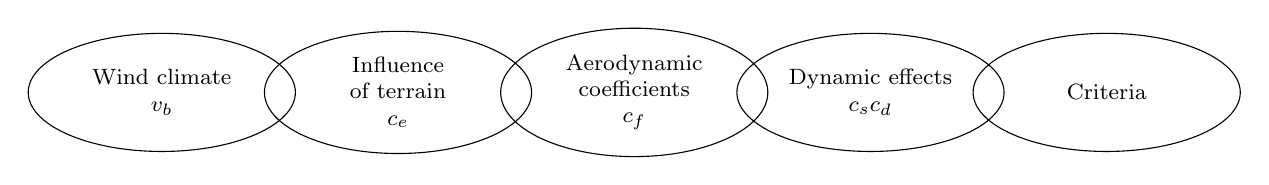
\begin{tikzpicture}[node distance = 3 cm, auto]
% tikz settings
\footnotesize
\tikzstyle{block} = [ellipse, draw,  
    text width=2.2cm, text centered,  rounded corners ,minimum height=1.5cm]
\tikzstyle{line} = [draw, latex-latex]

% the tikz picture
\node [block, align=center] (windclimate) {Wind climate \\ $v_b$};
\node [block, align=center, right of=windclimate] (influenceofterrain) {Influence of terrain \\ $c_e$ };
\node [block, align=center, right of=influenceofterrain] (Aerodynamic) {Aerodynamic coefficients \\ $c_f$};
\node [block, align= center, right of=Aerodynamic] (Dynamic) {Dynamic effects \\ $c_sc_d$};
\node [block, align=center, right of=Dynamic] (criteria) {Criteria};
\end{tikzpicture}
\caption{Davenport Wind Loading Chain, based on  \cite{Davenport_2002}}
\end{figure}

\noindent
For a propor representation of the structural reliability, the uncertainties in each of the links in the DWLC as well as the effects of wind-directionality need to be discounted for in the reliability analysis \cite{Davenport_1983b}. However, both the probabilistic modeling of the individual links in the chain, as well as methods to deal with wind-directionality effects, are still under active debates in the scientific cummunity. Besides, only a limited number of research exists that provides a full-probabilistic assessment of wind-loaded structural elements. \\
\\
In the following sections, an overview is presented of the most important findings regarding the probabilistic modeling of the individual links in the DWLC (see SECTION), the probabilistic methods for taking into account wind directionality effects (see SECTION) and the published results regarding full-reliability calculations (see SECTION). In section SECTION a motivation of out modeling choices is presented.



\subsection{Probabilistic modeling of of DWLC components}
Most of these discussions are related to the probabilistic modeling of the 'wind climate' and the 'aerodynamic coefficients', whilst little attention is directed towards the probabilistic modeling of the 'influence of terrain'. The reason for this is twofold. First, the 'influence of terrain' is assumed to have a lesser contribution to the total wind load effect than the other two \cite{} and second, data regarding the 'influence of terrain' are scarse. Consequentially, the probabilistic modeling of the 'influence of terrain' generally occurs on the basis of the probabilistic model code \cite{PMC, Hansen_2015} or on the basis of expert knowledge \cite{Sedlacek}.\\
\\
Both the probabilistic modeling of the 'wind climate' and 'aerodynamic coefficients' regard the probabilistic modeling of extremes. 
The discussions in both links therefore have many similarities. The main points of discussion thereby are (1) the extremal analysis method and distribution type to be used for the modeling and (2) the parameter interference techniques to be applied for the distribution fitting. Both issues will be addressed below. 



\subsubsection{Extremal analysis method (and distribution type)}
The extreme wind speeds and the extreme pressure coefficients are generally modeled on the basis of measurement data in combination with extremal analysis methods. 
Literature provides a numerous amount of extremal analysis methods and distribution models for the probabilistic modeling of extremes. Roughly, these methods can be distinguished in block maxima methods (BM), and the Peak over Theshold methods, and extensions to these methods. In \cite{Palutikov} an overview is provided of applications of these methods on wind speeds. In \cite{} an overview is provided of applications of these methods on pressure coeficients. \\
\\
\textit{Block maxima methods}\\
The basis of the BM methods lies in the division of the observation period into nonoverlapping blocks (periods of equal size) and restricts attention to the maximum observation in each block, over which an extreme value distribution is fitted. The main assumptions of the BM method are independent and identically distributed (i.i.d) random variables and convergion of the parent distribution towards the Generalized Extreme Value distribution (GEV). \\
\\
Within wind engineering, discussions regarding  the BM method are related to (1) the minimum block-duration to ensure statistically independent extremes and (2) which extreme value distribution to fit on the extremes. 
\begin{itemize}
\item In the case of extreme wind speeds, the block-duration is gerenally chosen to be one year. The main reason for this is to capture seasonal effects, rather than to ensure statistically independency. A more pronounced discussion exists regarding the distribution type to fit on the extremes. Traditionally the Gumbel distribution is taken. The theoretical justification of this distribution lies in the widely accepted assumption that the parent wind speeds are distributed by the reversed two parameter Weibull distribution, of which the extremes converge towards the Gumbel distribution \cite{Cook,Gumbel?}. However, based on Pickands GPD model estimation\cite{} and domain of attraction discrimination \cite{} \cite{Lechner_1992} compared the results of 100 US-wind records and found that in 61 cases the Weibull (W2/3?) distribution was the best fit, 36 the Gumbel distribution and in 3 cases the Frechet distribution was the best fit. Gomez and Vickery state that, in cases of mixed climates, the Fr\'{e}chet distribution is the best.

\item In the case of the extreme pressure coefficients the minimum required block-duration is less of a settled issue. Cook and Mayne [1] based the minimum record-length on the lower limit of the Spectral Gap in the Macrometeorological spectrum and suggested that one record should have a minimum length of 10 minutes. Lou and Peterka [4] used signal autocorrelation as a measure of dependency between extremes and found that periods smaller than 1 minute would already suffice. A recent study \cite{Meinen_2015} showed that the sample duration could be shortened to 10 seconds. Comparisons of the effect of different block-durations on the level of the Cook-Maybe fractile may be found in the literature as well \cite{Cook}\cite{Gavanski_2013}\cite{Peng201411} \cite{Quan_2014} and found that the results were significant. \\
\\
The type of Extreme Value distribution that should be fitted on the extreme pressure coefficients is neither a settled issue. In most  cases the Gumbel distribution is fitted. Kasperski however \cite{Kasperski2003527} discusses the use of the upper-bounded Weibull distribution, for reasons that wind tunnels cannot produce unlimited pressures for a given mean wind speed. Based on a statistical analysis of measurement data, he finds that in most of the cases indeed the W2/3 distribution best fits the data and in some cases the Frechet or Gumbel distribution. Similar findings are made by other researchers \cite{Holmes2003893, Quan_2014}. 
\end{itemize}

\textit{POT method}\\
In the POT, one selects those of the initial observations that exceed a certain high threshold after which the
Pareto distribution is fitted \cite{Pickands_1975}. Main discussions are related to the height of the threshold value and the methods to ensure statistically independent extremes. 
\begin{itemize}
\item POT and extreme wind speeds?
\item POT and extreme pressure coefficients?
\end{itemize}

\subsubsection{Distribution parameter interference techniques}
\added[id=NEM]{By arpad}\\
Some papers addressing the importance of sampling errors on the design wind speeds:
\begin{itemize}
\item Simiu \textit{et. al} \cite{Simiu_1978} investigated (among others) the effects of sampling errors on the estimation of design wind speeds from a confindent interval approach and found them to be significant.
\item 
Rojiani and Wen \cite{Rojiani_1980} also (among others) investigated the effects of sampling uncertainties on the design wind speeds and found that the effects of distribution type and parameter esitmation technique were of larger signifance. 
\end{itemize}

\subsection{Wind directionality}
Several researchers have investigated the influence of wind-directionality on the design wind loads. \\
Simiu and Filiben \cite{Simiu_1981} show that "cladding loads calculated without taking directional information on extreme wind speeds into account may in certain cases be larger than the actual loads by a factor of two or more." \\
Isyumov \textit{et. al} \cite{Isyumov_2014} state that "the ASCE 7 directional factor of Kd=0.85 is not unreasonable for the structural and cladding loads for buildings located in areas, where extra-tropical winds dominate." \\
Davenport \cite{Davenport_1983b} estimated the differences in the risks in the design of cladding pressures when the influence of wind direction is taken into account and found that "if the peak pressure coefficient aligns with a direction of relatively weak winds, the reduction can easily be a factor two". 

\subsection{Full probabilistic analysis}
As stated before, the focus of the literature is mostly on the in-depth analysis of a single, selected link only. In the literature, a handful of studies may be found that provide a full-probabilistic assessment which accounts for the uncertainties in the entire DWLC.  \\
\\
The ones were Cook and Mayne \cite{Mayne1979109}, who developed a method \added[id=NEM]{often referred to as 'the Simplified Method'} to account for the uncertainties in the wind speeds and the pressure coefficients, where the uncertainties in the other links were kept deterministic.  Many researchers \cite{Kasperski2003527,Harris_2003} have used, discussed and refined this method.\\
\\
Some recent studies did account for the uncertainties in all links jointly. \\
E.g. for the purpose of partial factor calibration Hansen \cite{Hansen_2015} and Sedlacek provide a full probabilistic design method that takes into account uncertainties in all links. For the probabilistic modeling of each of the parameters choices were made based on literature / sample data. The effects or their modeling choices on the reliability level were however not investigated. \\
\\
In a super amazing pioneer study \added[id=NEM]{just kidding}, Meinen investigated the influence of some modeling choices ont he reliability level of an element. The results showed that.. ? It is actually interesting to look at the influence of modeling choices on beta-level, as it has a large impact. \\
\\
As a result, only limited knowledge exists on the effects of modeling choices on the structural reliability of wind-loaded structural elements, i.e. uncertainty propagation.



\subsection{Our choices with respect to the modeling of extremes}
As it it 

In this research the block-method combined with the Generalized Extreme Value distribution is adopted \cite{CUR_103} \cite{Kasperski2003527} \cite{Holmes2003893}. 





\end{document}


%\documentclass[fleqn]{article}
%\usepackage{graphicx} 
%\usepackage{here}    
%\usepackage{amsmath}
%\textwidth=15.0cm
%\textheight=22.0cm
%\topmargin=-1cm
%\oddsidemargin=-0.3cm
%\evensidemargin=-0.3cm
%
%
%%packages
%\usepackage{amsmath}
%\usepackage{cite}
%\usepackage[toc,page]{appendix}
%\usepackage{fancyvrb}
%\usepackage{tikz}
%\usepackage{multicol}
%\usepackage{framed}
%\usepackage{pgfplots}
%\usepackage{fixltx2e}
%\usepackage{subfigure}
%\usepackage{lscape}
%\usepackage{enumitem}
%\usepackage{multirow}
%\usepackage{color}
%\usepackage{xcolor}
%\usepackage{comment}
%\usepackage{changes}
%\renewcommand*\descriptionlabel[1]{\hspace\leftmargin$#1$}
%
%%tikz labraries
%\usetikzlibrary{matrix}
%\usetikzlibrary{decorations.pathreplacing}
%\usetikzlibrary{positioning}
%\usetikzlibrary{calc}
%\usetikzlibrary{shapes,arrows, chains}
%\usetikzlibrary{intersections}
%\usetikzlibrary{decorations.markings}
%\usetikzlibrary{calc,intersections}
%\usetikzlibrary{patterns}
%
%
%\makeatletter
%\def\mathcolor#1#{\@mathcolor{#1}}
%\def\@mathcolor#1#2#3{%
%  \protect\leavevmode
%  \begingroup
%    \color#1{#2}#3%
%  \endgroup
%}
%\makeatother
%
%%##### DEFINE YOUR NAME #########################
%\definechangesauthor[color=blue,name={Arpad Rozsas}]{AR}
%\definechangesauthor[color=red,name={Nadieh Meinen}]{NEM}
%%###########################################
%
%\begin{document}

\section{Methodology}


\subsection{Overview}

\begin{itemize}
\item
The importance assessment will be conducted trough the reliability of a generic structural member. 

\item
For this, first the structural resistance is determined by design according to codes. Choice of probabilistic models. This is further explained in SECTION. 

\item
Subsequently the load effects on the structural member are determined on the basis of literature and measurement data. Choice of probabilistic models need to be made. Different models will exist for different incident wind directions. See SECTION. 

\item 
Subsequently limit state function. These need to be made for each incident wind direction.  Furthermore it needs to be accounted for both faiolure modes: failure due to suction and failure due to compression. 

\item 
Subsequently it needs to be accounted for the system effects. Thereby it is assumed that it is a system that can fail due to wind coming from different incident wind directions. It needs to be accounted for correlations in the wind speed parameters as well as the resistance parameters.

\item 
Final beta-value used for comparison. 

\end{itemize}


\subsection{Limit state function}
\begin{framed}
Should we add here something like general principles regarding reliaiblity analysis? E.g. explanation of limit state functions etc. such as in Sedlacek? Then we could use something like that as an introduction to the methods used?
\end{framed}

\subsection{Load effect model}

\subsubsection{Davenport Wind Loading Chain}





\subsubsection{Adopted physical model}
Though most codes of practice rely on the concepts of the DWLC, the numerical completion of the wind load model may be different for different codes.  

Much effort has been put to put it into model. Often for the modeling of the fluctuations and such the quati-steady wind model where it is assumed that the pressures on the building surface follow  the variations in upwind velocity, i.e. it is assumed that a peak value of wind speed is accompanied by a peak value of pressure or load on the structure. \\
\\
The quasisteady model has been found to be fairly reliable for wind loading on small structures and is used in codes and .. \\

WHERE DID I FIND THIS??
\begin{framed}
In most current design codes this is based on a WMO mean wind speed with a specified probability of occurrence. All countries that are members of the WMO produce wind statistics in the form of mean wind speeds taken over an averaging time of between 10 min and 1 h. In the UK an averaging period of an hour is used so, for convenience in all that follows, means will be described as hourly means, with the understanding that in other countries where a different averaging period is used, that average is implied. If another WMO averaging period is being used then some of the numerical constants that appear in the paper may need to be amended, however the results will not be influenced by that. 
\end{framed}
In current codes of practice, wind loads are treated as quasi-static loads. \\
In this study, the general physical model is elaborated as follows. The model is based on the EN1991-1-4 action model for static (local) wind loads, however with the following adaptations:
\begin{itemize}
\item reformulated such that one can make use of peak external pressure coefficients obtained from wind tunnels
\item reformulated such that the reference wind speeds does not necessarily belongs to the specified characteristics in the EC
\item change of averaging time not 10 minutes but more general, lets say T. 
\end{itemize}
This means that the wind load per unit area becomes: 
\begin{equation}\label{eq:wind_loads}
S(\theta) = \frac{1}{2}\rho \bar{v}_T(\theta)^2 \cdot c_r(z, z_0(\theta), z_{ref})^2 \cdot  \hat{c}_{pe,T}(\theta) 
\end{equation}
Where\\
\vspace{0.2cm}
\begin{tabular}{l l}\\
$\theta$ & is the incident wind direction with respect to the north\\
$S$ & is the extreme wind load with a certain reference period [N]\\
$\rho$ &  is the air density [kg/m$^3$]\\
$\bar{v_T}$ & is the $N$-yearly extreme mean wind speed under standard terrain averaged over time T [m/s] with reference period $N$ \\
$c_r(.)$ & is the roughness factor correcting for height and terrain roughness\\
$z$ & the height on the structure [m]\\
$z_0$ & is the terrain roughness  [m] \\
$z_{0,ref}$ & is the reference terrain roughness for which the wind speeds are corrected [m]\\
$\hat{c}_{pe,T}$ & the peak external pressure coefficient within time $T$ at the location of interest [-]\\
\end{tabular}


\subsubsection{Probabilistic model}
Davenport states that the uncertainties in each of the links need to be taken into account probabilistically. He does however not state which if the elements within each of the links that should be. \\
\\
Key task is therefore to identify which of the components in there contribute most to the uncertainties in each of the links, and which may be kept deterministic. \\
\\
Guidance is provided in \cite{Kasperski_PAPER}. Also another earlier research \cite{meinen} has pointed the most relevant sources of uncertainties in the design of static elements loaded by local wind loads. The choice was made on:
\begin{itemize}
\item relative importance
\item availability of literature / measurement data. 
\end{itemize}
This means that the following parameters in the wind load model shall be modeled probabilistically, others are kept deterministic:
\begin{itemize}
\item extreme reference averaged pressures
\item the peak external pressure coefficients
\item the terrain roughness factor as a whole 
\item model uncertainty factors \added[id=NEM]{is not yet introduced though}
\end{itemize}
In the next sections it will be explained how they will be modeled exactly. 

\begin{framed}
Key assumptions of our probabilistic approach 
\added[id=NEM]{I haven't found a place for it yet.}
\begin{itemize}
\item Elements are statistically independent (generally assumed, rectiefied by Cook and Mayne
\item Peak load occurs when peak pressures and peak windspeeds come together. Corrections to this thought can be found in.. Harris etc. Dont know whether that is relevant to mention. 
\end{itemize}
\end{framed}


\paragraph{Extreme wind speeds}
For the modeling of extreme wind speeds / pressures use measurement data are being used. These measurement data consist of instantaneous T-averaged mean reference wind speeds with accompanying discretized incident wind directions. For convenience these are called the parent data in the following.
\begin{itemize}
\item 
\textit{Directionality effects}\\
As a consequence of wind directionality (caused by different underlying physical phenomena) the following important things need to be taken into account :
\begin{itemize}
\item 
wind speed characteristics differ for different incident wind directions 
\item 
probabability of wind coming from a certain incident direction not uniformly distributed among the Wind Rose.
\item 
dependencies between (adjacent) (extreme) wind speeds
\end{itemize}
In the litarature a lot of discussion going on on the appropriateness of methods to take into account upper effects. See for example \cite{Morarty_1983} and \cite{Isyumov2014169}.\\
\\
In this research we apply the following method (SEARCH?). \added[id=NEM]{When to introduce the disadvantages?}\\
The parent data are sub-divided into direction-dependent parent data. The probabilistic descriptions of the direction-dependent extreme wind speeds occur on the basis of these parent wind data. \\
\\
The probability of the incident wind coming from direction $\theta_i$ is estimated by the proportion of measurements coming from incident wind direction $\theta$, divided by the total number of wind speed measurements, i.e.:
\begin{equation}
P(\theta)=\frac{Nr(\theta)}{Nr}
\end{equation} 
The correlation between adjacent (extreme) wind speeds are taken into account by pierson correlation coefficient....  

\begin{framed}
Still say something like that we are going to apply a distribution function on each of these directional extremes - or is that unnecessary? 
\end{framed}



\item
\textit{Distribution type and method}\\
For the modeling of the extreme wind speeds the BM is applied with annual maxima. Thereby yearly extremes are obtained, distribution function is fitted and statistically extrapolated to larger return periods \added[id=NEM]{should we mention the formulas?}. Two distribution functions are applied. The Gumbel distribution and the W3 distribution. The used parametrisation of the distribution functions may be found in APPENDIX. \\
\\
Two remarks:
\begin{itemize}
\item The same method / distribution function will be applied for all incident wind directions without checking its appropriateness.
\item the applied method for wind directionality is not perfect due to masking of gusts, see \cite{Moriarty_DIRECTIONALITY}. 
\end{itemize}

\item 
\textit{Distribution parameter estimation}\\
In this research for the parameter estimation the MLE method is being ised. \\
\\
Also effects of sampling uncertainties are taken into account. \\
\\
A lot of methods exist for that.\\
\\
Here we use the Bayesian method. \\
\\
Application of that see PAPER ARPAD.\\
\\
Prior distributions that are assumed are ....
\end{itemize}


\paragraph{Extreme pressure coefficients}
On the basis of the probabilistic description of the direction-dependent hourly extreme peak external pressure coefficients lie instantaneous wind tunnel measurements which are processed to dimensionless pressure coefficients. Generally the wind tunnel measurements are performed for different incident wind directions. 
\begin{itemize}
\item
\textit{Wind directionality and flow around the building}\\
Depending on the incident wind-direction different flow phenomena may occur around the building, that, depending on the location on the building, either resulting in high pressure (represented by the maximum peak external pressure coefficients $\hat{c}_{pe}$), high suction (represented by the minimum peak external pressure coefficients $\check{c}_{pe}$) or both. 

\added[id=NEM]{We have to think about whether we think there is correlation between maxima / minima and correlation between (adjacent) extremes and if so, how to take that into account in the reliability analysis.}

\item 
\textit{Extremal analysis method and distribution function}\\
See wind speeds, similar description. \\
\\
State that a lot of discussion is going on on block-duration versus number of samples and refer to some of these discussions.  
State that our choice of block-duration and nr of sdamples is going to be based on CUR-guidelines meaning at least ... number of 60s-extremes. This was also as proposed by Cook and Mayne based on theoretical considerations. Alternative methods are autocorrelation method from CITE. \\
\\
Two remarks:
\begin{itemize}
\item Except for papers focussing on the determination of block-duration vs. nr of sample data papers almost NEVER mention how they got their distribution functions of the pressure coefficients. 
\end{itemize} 


For practical implementation the described statistical method is adopted for each incident wind-direction $\theta_i$. 

\item
\textit{Parameter estimation technique}
\added[id=NEM]{Should we make this a part of parameter estimation technique?}
\end{itemize}

\paragraph{Roughness factor}
The roughness factor accounts for that and that. For the upwind terrain. The roughness factor is therefore a function of incident wind directionality.\\
\\
No probabilistic model exist on the level of the terrain roughness. However, accoridng to PMC, rouighness factor can lie between that and that with a mean to \\
\\
The Probabilistic Model Code on wind loads provides first estimates on the probabilistic modeling of the roughness factor / exposure factor. \\
\\
It is remarked that here the roughness factor is called exposure factor. \\
\\
Here the roughness factor squared is modeled by a two-parameter lognormal distribution, with a mean value of $\mu=0.8*c_{r,s}(\theta_i)^2$ and a coefficient of variation of V=0.15 [-]. \\
It is remarked that in this approach it is assumed that the COV of the roughness as well as the distribution type is independent of the height of interest. \\
\\
To find out the influence of these choices.. the roughness factor will be subject to a parametric analysis for COV between 0.1 en 0.2. \\
\\
Here $c_{r,s}(\theta_i)^2$ represents the specified roughness factor according to the code. In this case the EC. \\
\\
Two remarks regarding this:
\begin{itemize}
\item My opinion: this value of 0.8 is super random. I think it belongs to the NBCC only and I think such a statements cannot really be generalized to all other builing codes just like that. How to state this?
\end{itemize}


\subsubsection{Model uncertainties}
\begin{framed}
In what will we vary here? Both in variance and distribution type? Or not at all... also fine by me? Does it make sense to vary these things here or should we better focus on other things?
\end{framed}
\begin{itemize}
\item \textit{Uncertainty in the load-model}\\
As stated bty Davenport, the wind loading chain is a quasi-static approach of the sitaution. This .. goes with the cost of model uncertainties within the wind load model. These are accounted for by the addition of a model uncertainty factor theta model.

The model uncertainty factor $\chi_{model}$ is modeled by a normal distribution with mean $\mu=1$ [-] and coefficient of variation  V = 0.2 [-]. 

Furhtermore there is the load effect thing that translates loads to load effects, i.e. pressures in the structural component. 
The load effect uncertainties include approximation of the models assumed for the load and for the load effect calculation. 



\item \textit{Uncertainty in the load-effect model}\\
The uncertainties in the load effect are related to... The uncertainties are related to the failure mode under consideration.\\
\\
PMC gives handles to these uncertainties. \\
Are eual to .. for steel in bending and .. for .. 

\end{itemize}


\subsubsection{Standards}
Standards have also design values of the loads and load effects. To obtain the design value of the wind load use is made of the EC. For the exact values of these loads see appendix, there it is elaborated for the EC. 

\subsection{Resistance model}


\subsubsection{Physical model}
The actual resistance model depends on the material type and failure mode considered. In this research a generic steel member is assessed. 
The physical model for a generic steel member can be written like:

\begin{equation}
R = \theta_{\mathrm{R}} A f_{\mathrm{y}}
\end{equation}
Where:\\
\vspace{0.2cm}
\begin{tabular}{l l}
$A$ & is the effective area of the steel member [mm$^2$] \\
$f_{\mathrm{y}}$ & is the yield stress of the steel [N/mm$^2$]
\end{tabular}

\subsubsection{Probabilistic model}

\begin{equation}
R = \theta_{\mathrm{R}} A f_{\mathrm{y}}
\end{equation}
Where:\\
\vspace{0.2cm}
\begin{tabular}{l l}
$\theta_{\mathrm{R}}$ & is the model uncertainty for the resistance model \\
$A$ & is the effective area of the steel member [mm$^2$] \\
$f_{\mathrm{y}}$ & is the yield stress of the steel [N/mm$^2$]
\end{tabular}

Each of the factors should be modeled probabilistically. For this see TABLE. 

\subsubsection{Partial factor design of a steel member}
Most codes work with partial factor design. This works as follows.\\ 
\\
The design resistance of a generic steel member may be expressed by the following relationship [SEDLACEK]:
\begin{equation}
R_{\mathrm{d}} = a\frac{f_{\mathrm{k}}}{\gamma_{\mathrm{M}}}
\end{equation}
Where $a$ denotes a design parameter depending ont he geometry and boundary conditions of the memberm $f_{\mathrm{k}}$ denotes the characteristic strength of the member and $\gamma_{\mathrm{M}}$ denotes the partial factor of the (uncertain) material property (WHAT IS MEANT BY THAT?). \\
\\
In case of optimal design, the design value of the structural resistance is equal to the design value of the load effects, i.e.:
\begin{equation}
R_d = E_d
\end{equation}
Where $E_d$ is determined as described above. \\
\\
Based on this knowledge, the minimum required design parameter can be determined by substituting.. and then rewriting:
\begin{equation}
a = \frac{ E_{\mathrm{d}} \gamma_{\mathrm{M}}} {f_{\mathrm{k}}} 
\end{equation}
Depending on the material property, the partial factor is normally within the interval of $\gamma_{M}=[1; 1.15]$.\\ 
\\
This also includes the model uncertainty thiung... 


\subsection{Reliability analysis}

REGARDING THE SYSTEM EFFECTS. 
The direction-dependent failure probability $P_f(\theta_i)$ can be obtained by the summation of the failure probability caused by high pressure together with the failure probability caused by high suction. Therefore both the extreme maxima and extreme minima are of interest. These are indicated by... hat and non-hat.

%\begin{figure}
%\centering
%\documentclass[fleqn]{report}
\usepackage{graphicx} % om PostScript plaatje in te lassen
\usepackage{here}     % voor geforceerde plaatsing figuren
\usepackage{amsmath}
\textwidth=17.0cm
\textheight=22.0cm
\topmargin=-1cm
\oddsidemargin=-0.3cm
\evensidemargin=-0.3cm

%packages
\usepackage{amsmath}
\usepackage{cite}
\usepackage[toc,page]{appendix}
\usepackage{fancyvrb}
\usepackage{tikz}
\usepackage{multicol}
\usepackage{framed}
\usepackage{pgfplots}
\usepackage{fixltx2e}
\usepackage{subfigure}
\usepackage{lscape}
\usepackage{enumitem}
\usepackage{filecontents}

%tikz labraries
\usetikzlibrary{matrix}
\usetikzlibrary{decorations.pathreplacing}
\usetikzlibrary{positioning}
\usetikzlibrary{calc}
\usetikzlibrary{shapes,arrows, chains}
\usetikzlibrary{intersections}
\usetikzlibrary{decorations.markings}
\usetikzlibrary{calc,intersections}
 \usetikzlibrary{svg.path}
 \usetikzlibrary{patterns}
\usepackage{xcolor}
%\usetikzlibrary{decorations.pathreplacing,bending}

%extra instellingen
\newlist{aims}{enumerate}{1}
\setlist[aims,1]{
  label={*},
  leftmargin=*,
  align=left,
  labelsep=2mm,
}

\newlist{aims2}{enumerate}{1}
\setlist[aims2,1]{
  label={},
  leftmargin=0pt,
  align=left,
  labelsep=4mm,
}

\newlist{aims3}{enumerate}{1}
\setlist[aims3,1]{
  label={-},
  leftmargin=2cm,
  align=left,
  labelsep=0.4mm,
}

\usepackage{pgfplots}

\begin{document}


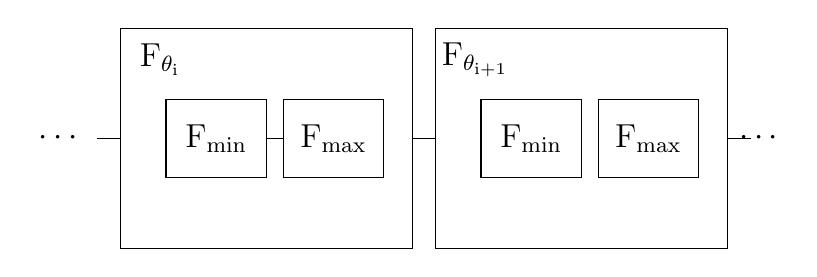
\begin{tikzpicture}
\footnotesize

% used shapes
\tikzstyle{block} = [rectangle, draw, node distance = 0.2cm, text width=1cm, text centered, minimum height=1cm]
\tikzstyle{diamond_thing} = [diamond, draw, node distance = 0.5cm, text centered, minimum height=1cm]
\tikzstyle{blokje} = [rectangle, draw, rounded corners = 5pt, node distance = 0.5cm, text width=2cm, text centered, minimum height=0.5cm,fill=purple!20]
\tikzstyle{blockrounded} = [rectangle, draw, rounded corners = 5pt, node distance = 1cm, fill=yellow!20, text width=3cm, text centered, minimum height=0.5cm]
\tikzstyle{blockroundedred} = [rectangle, draw, rounded corners = 5pt, node distance = 1cm, fill=red!20, text width=3cm, text centered, minimum height=0.5cm]

\large

\draw (-3,0) -- (-2.7,0);
\draw (-2.7,-1.4) rectangle (1,1.4);

\node at (-2.2, 1) {$\mathrm{F}_{\mathrm{\theta_i}}$};

\node [block] (max)  {$\mathrm{F}_{\mathrm{max}}$};

\node [block, left = of max] (min)  {$\mathrm{F}_{\mathrm{min}}$};

\draw (min) -- (max);

\begin{scope}[shift={(4,0)}]
 \draw (-3,0) -- (-2.7,0);
\draw (-2.7,-1.4) rectangle (1,1.4);

\node at (-2.2, 1) {$\mathrm{F}_{\mathrm{\theta_{i+1}}}$};

\node [block] (max)  {$\mathrm{F}_{\mathrm{max}}$};

\node [block, left = of max] (min)  {$\mathrm{F}_{\mathrm{min}}$};

\end{scope}



\draw (5,0) -- (5.3,0);

\node at (-3.5, 0) {$\mathbf{\cdots}$};
\node at (5.4, 0) {$\mathbf{\cdots}$};

\end{tikzpicture}





\end{document}
%\caption{\added[id=NEM]{Something like this to visualize how we incorporated system effects - maybe include also correlations or something}}
%\end{figure}

\subsubsection{System effects}
A structural member can fail due to incident wind coming from different incident wind directions. Thereby there exists a certain corerlation between the (extreme) wind speeds from adjacent incident wind directions. \\
\\
Furthermore, within a certain incident wind direction, a structural member can fail due to either high compression forces or high suction forces.\\
\\
This means that the failure of a structural element may be modeled as a series system consisting of several elements - each for a certain incident wind directions - which are built up out of each two elements what are also a series system. This is displayed in figure FIGUIRE. 


Given a certain incident wind direction

\begin{itemize}
\item by assuming a series system, i.e. when it fails due to incident wind from one direction then the thing has failed
\item accounting for correlation in the resistance by implementation of correlation... pierson etc.
\item it is assumed that there is no correlation between failure due to suction and failure due to compression
\item assumption no correlation on the loading side? Or shall we just use obtained piersons for that based on measurement data?
\end{itemize}

\subsubsection{Limit state function}
\begin{framed}
Already introduct direction-dependent limit state function?
\end{framed}
Starting point of the reliability analysis is 
a specific design situation describing all input parameters relevant for the design of the wind loaded structural member.  These include design parameters with respect to the structural resistance, $X_R$, and design parameters with respect to the loads, $X_S$. 

The limit state function is related to the failure mode under consideration. It separates .. states from adverse states. 
The general limit state function that will be used here is:

\begin{equation}
Z = R(X_r, \theta_R) - E(X_s, \theta_E)
\end{equation}
Where $\theta$ are model uncertainties. 


\begin{framed}
How are we going to introduce wind directionality here? The letter i indicates the specific incident wind direction??
\end{framed}


In case all the probabilistic models of all the stochasstic random variables have been oftained the reliability calculation can be performed. 
\begin{itemize}
	\item FROM reliability calculation
	\item How system effects are taken into account / correlation etc.
	\item Limit state functions
\end{itemize}





%\end{document}


%\documentclass[fleqn]{article}
%\usepackage{graphicx} 
%\usepackage{here}    
%\usepackage{amsmath}
%\textwidth=15.0cm
%\textheight=22.0cm
%\topmargin=-1cm
%\oddsidemargin=-0.3cm
%\evensidemargin=-0.3cm
%
%
%%packages
%\usepackage{amsmath}
%\usepackage{cite}
%\usepackage[toc,page]{appendix}
%\usepackage{fancyvrb}
%\usepackage{tikz}
%\usepackage{multicol}
%\usepackage{framed}
%\usepackage{pgfplots}
%\usepackage{fixltx2e}
%\usepackage{subfigure}
%\usepackage{lscape}
%\usepackage{enumitem}
%\usepackage{multirow}
%\usepackage{color}
%\usepackage{xcolor}
%\usepackage{comment}
%\usepackage{changes}
%\renewcommand*\descriptionlabel[1]{\hspace\leftmargin$#1$}
%
%%tikz labraries
%\usetikzlibrary{matrix}
%\usetikzlibrary{decorations.pathreplacing}
%\usetikzlibrary{positioning}
%\usetikzlibrary{calc}
%\usetikzlibrary{shapes,arrows, chains}
%\usetikzlibrary{intersections}
%\usetikzlibrary{decorations.markings}
%\usetikzlibrary{calc,intersections}
%\usetikzlibrary{patterns}
%
%
%\makeatletter
%\def\mathcolor#1#{\@mathcolor{#1}}
%\def\@mathcolor#1#2#3{%
%  \protect\leavevmode
%  \begingroup
%    \color#1{#2}#3%
%  \endgroup
%}
%\makeatother
%
%%##### DEFINE YOUR NAME #########################
%\definechangesauthor[color=blue,name={Arpad Rozsas}]{AR}
%\definechangesauthor[color=red,name={Nadieh Meinen}]{NEM}
%%###########################################
%
%\begin{document}


\section{Case study}\label{case_study}

\subsection{Design situation}
A graphical summary of the (fictitious) design situation is presented in Figure \ref{tikz:design_situation}. The design situation exists of a  high-rise structure of height  $h=120$ m and a square plan with measurements of $w=b=30$ m. The structure is located at Schiphol Airport. All possible building orientations $\phi$ are investigated. The surrounding terrain roughness is equal to $z_0=0.8$ m. The faces of the building are named A to D. Interest goes to the fa\c{c}ade element located in the middle of face A at the height of $z=80$ m. The size of the fa\c{c}ade element is equal to  $A_{ref}=10$ m$^2$. The fa\c{c}ade element is designed for the EN1990 consequence class 2 (e.g. residential and office buildings) with the minimum design lifetime of $N=50$ years. The target value of the reliability index is equal to $\beta=3.8$. The detachment system of the fa\c{c}ade element is manufactured from steel and is loaded in axial compression. The incident wind-directions are discretized into sections of 30$^{\circ}$. 


\begin{figure}[H]
	\centering
	\subfigure[Location of the structure]{
		%\documentclass[fleqn]{report}
%\usepackage{graphicx} % om PostScript plaatje in te lassen
%\usepackage{here}     % voor geforceerde plaatsing figuren
%\usepackage{amsmath}
%\textwidth=17.0cm
%\textheight=22.0cm
%\topmargin=-1cm
%\oddsidemargin=-0.3cm
%\evensidemargin=-0.3cm
%
%%packages
%\usepackage{amsmath}
%\usepackage{cite}
%\usepackage[toc,page]{appendix}
%\usepackage{fancyvrb}
%\usepackage{tikz}
%\usepackage{multicol}
%\usepackage{framed}
%\usepackage{pgfplots}
%%\usepgfplotslibrary{fillbetween}
%\usepackage{fixltx2e}
%\usepackage{subfigure}
%\usepackage{lscape}
%\usepackage{enumitem}
%\usepackage{filecontents}
%\usetikzlibrary{decorations.pathmorphing}
%\usepackage{lmodern}
%\usepackage{pgfplotstable}
%
%\usetikzlibrary{arrows}
%%\usetikzlibrary{arrows.meta}
%
%
%
%\usetikzlibrary{decorations.pathreplacing,decorations.markings,snakes}
%
%%tikz labraries
%\usetikzlibrary{matrix}
%\usetikzlibrary{decorations.pathreplacing}
%\usetikzlibrary{positioning}
%\usetikzlibrary{calc}
%\usetikzlibrary{shapes,arrows, chains}
%\usetikzlibrary{patterns}
%
%\usetikzlibrary{intersections}
%\usetikzlibrary{decorations.markings}
%\usetikzlibrary{calc,intersections}
%%\usetikzlibrary{decorations.pathreplacing,bending}
%
%%extra instellingen
%\newlist{aims}{enumerate}{1}
%\setlist[aims,1]{
%  label={*},
%  leftmargin=*,
%  align=left,
%  labelsep=2mm,
%}
%
%\newlist{aims2}{enumerate}{1}
%\setlist[aims2,1]{
%  label={},
%  leftmargin=0pt,
%  align=left,
%  labelsep=4mm,
%}
%
%\newlist{aims3}{enumerate}{1}
%\setlist[aims3,1]{
%  label={-},
%  leftmargin=2cm,
%  align=left,
%  labelsep=0.4mm,
%}
%
%\usepackage{pgfplots}
%
%\begin{document}


\begin{tikzpicture}[scale=2]
\small 
\node [above right] (Nederland) at (0,0) {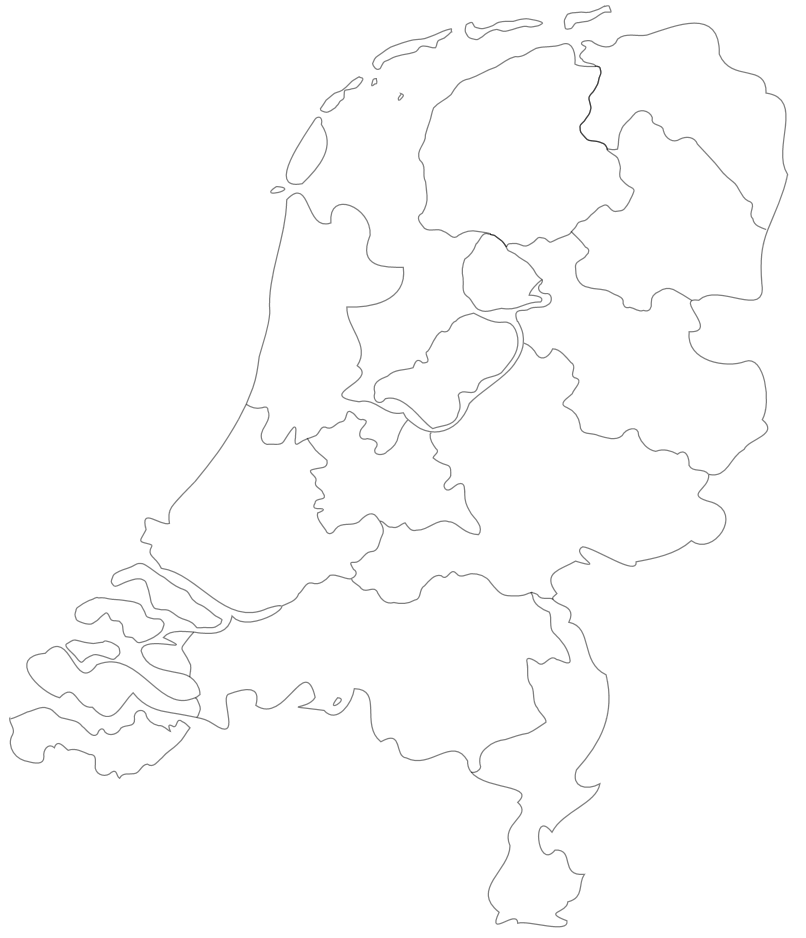
\includegraphics[height=4cm]{tikz/images/Nederland}};
\begin{scope}

\coordinate (schiphol) at (0.7,1.2);
\coordinate (vlissingen) at (0.15,0.57);
\coordinate (eindhoven) at (1,0.52);
%\coordinate (debilt) at (0.85, 1.0);

%\node [above](Eindhoven) at (eindhoven) {Eindhoven};
\node [above](Schiphol) at (schiphol) {Schiphol Airport};
%\node [above] (Vlissingen) at (vlissingen) {Vlissingen};
%\node [above](Debilt) at (debilt) {De Bilt};

\fill (schiphol) circle (0.2pt);
%\fill (eindhoven) circle (0.2pt);
%\fill (vlissingen) circle (0.2pt);
%\fill (debilt) circle (0.2pt);

\end{scope}



\end{tikzpicture}
%
%\end{document}
	}
	\subfigure[Location on the structure]{
		%
%\documentclass[fleqn]{report}
%\usepackage{graphicx} % om PostScript plaatje in te lassen
%\usepackage{here}     % voor geforceerde plaatsing figuren
%\usepackage{amsmath}
%\textwidth=17.0cm
%\textheight=22.0cm
%\topmargin=-1cm
%\oddsidemargin=-0.3cm
%\evensidemargin=-0.3cm
%
%%packages
%\usepackage{amsmath}
%\usepackage{cite}
%\usepackage[toc,page]{appendix}
%\usepackage{fancyvrb}
%\usepackage{tikz}
%\usepackage{multicol}
%\usepackage{framed}
%\usepackage{pgfplots}
%\usepackage{fixltx2e}
%\usepackage{subfigure}
%\usepackage{lscape}
%\usepackage{enumitem}
%\usepackage{filecontents}
%\usepackage{multicol}
%
%
%%tikz labraries
%\usetikzlibrary{matrix}
%\usetikzlibrary{decorations.pathreplacing}
%\usetikzlibrary{positioning}
%\usetikzlibrary{calc}
%\usetikzlibrary{shapes,arrows, chains}
%\usetikzlibrary{intersections}
%\usetikzlibrary{decorations.markings}
%\usetikzlibrary{calc,intersections}
%%\usetikzlibrary{decorations.pathreplacing,bending}
%
%% define mathcolor
%\makeatletter
%\def\mathcolor#1#{\@mathcolor{#1}}
%\def\@mathcolor#1#2#3{%
%  \protect\leavevmode
%  \begingroup
%    \color#1{#2}#3%
%  \endgroup
%}
%\makeatother
%
%%extra instellingen
%\newlist{aims}{enumerate}{1}
%\setlist[aims,1]{
%  label={*},
%  leftmargin=*,
%  align=left,
%  labelsep=2mm,
%}
%
%\newlist{aims2}{enumerate}{1}
%\setlist[aims2,1]{
%  label={},
%  leftmargin=0pt,
%  align=left,
%  labelsep=4mm,
%}
%
%\newlist{aims3}{enumerate}{1}
%\setlist[aims3,1]{
%  label={-},
%  leftmargin=2cm,
%  align=left,
%  labelsep=0.4mm,
%}
%
%\usepackage{pgfplots}
%
%\begin{document}

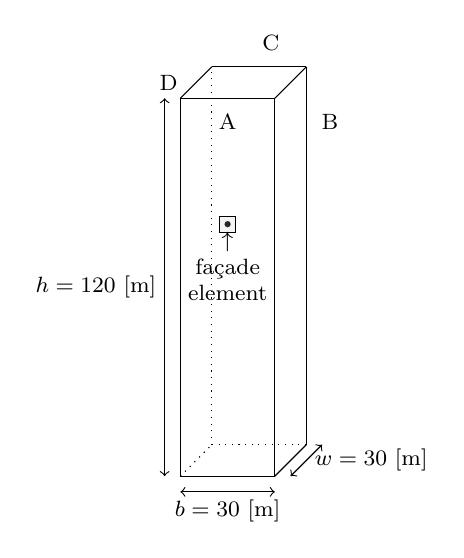
\begin{tikzpicture}[scale=10]
\footnotesize
\draw (-0.06,0) rectangle (0.06,0.480);
\draw (0.06,0) -- (0.10,0.04);
\draw (0.06,0.480) -- (0.10,0.52);
\draw (-0.06,0.480) -- (-0.02,0.52);
\draw (0.10,0.04) -- (0.10,0.52);
\draw (-0.02,0.52) -- (0.10,0.52);
\draw [dotted] (-0.06,0) -- (-0.02,0.04);
\draw [dotted] (-0.02,0.04) -- (0.1,0.04);
\draw [dotted] (-0.02,0.04) -- (-0.02,0.52);

% height
\draw [<->] (-0.08,0) -- (-0.08,0.480) node [midway, anchor=east] {$h = 120$ [m]};
% width
\draw [<->] (-0.06,-0.02) -- (0.06,-0.02) node [midway, anchor = north] {$b = 30$ [m]};
% depth
\draw [<->] (0.08,0) -- (0.12,0.04) node [midway, anchor = west] {$w = 30$ [m]};

%\draw [->] (-0.1,0) -- (-0.1,0.12);
%\node [left ] at  (-0.07,0.12) {$z$};
% x-distance
%\draw [<->] (-0.06,0.37) -- (0,0.37) node [midway, anchor = south] {x = 24 [m]};
% z-distance
%\draw [<->] (-0.03,0) -- (-0.03,0.32) node [midway, anchor = west] {$z = 80$ [m]};

\node at (0,0.45) {A};
\node at (0.13,0.45) {B};
\node at (0.055,0.55) {C};
\node at (-0.075,0.5) {D};
\draw (0,0.320) node[circle,fill,inner sep=0.8pt,align=center, label=below:]  (1) {};
\node [below, align=center] at (0,0.32) {$\uparrow$ \\ fa\c{c}ade \\ element};

\draw [fill=black!20, fill opacity=0.2] (-0.01,0.31) rectangle (0.01,0.33);


%\draw (-0.06,0.320) -- (0.06,0.32);
%\draw (0.06,0.320) --  (0.10,0.36); 


\end{tikzpicture}
%
%\end{document}
		\label{tikz:C_Okkebuilding_3D}
	}
	\subfigure[Orientation of the structure]{
		%
%\documentclass[fleqn]{report}
%\usepackage{graphicx} % om PostScript plaatje in te lassen
%\usepackage{here}     % voor geforceerde plaatsing figuren
%\usepackage{amsmath}
%\textwidth=17.0cm
%\textheight=22.0cm
%\topmargin=-1cm
%\oddsidemargin=-0.3cm
%\evensidemargin=-0.3cm
%
%%packages
%\usepackage{amsmath}
%\usepackage{cite}
%\usepackage[toc,page]{appendix}
%\usepackage{fancyvrb}
%\usepackage{tikz}
%\usepackage{multicol}
%\usepackage{framed}
%\usepackage{pgfplots}
%\usepackage{fixltx2e}
%\usepackage{subfigure}
%\usepackage{lscape}
%\usepackage{enumitem}
%\usepackage{filecontents}
%\usepackage{multicol}
%
%
%%tikz labraries
%\usetikzlibrary{matrix}
%\usetikzlibrary{decorations.pathreplacing}
%\usetikzlibrary{positioning}
%\usetikzlibrary{calc}
%\usetikzlibrary{shapes,arrows, chains}
%\usetikzlibrary{intersections}
%\usetikzlibrary{decorations.markings}
%\usetikzlibrary{calc,intersections}
%%\usetikzlibrary{decorations.pathreplacing,bending}
%
%% define mathcolor
%\makeatletter
%\def\mathcolor#1#{\@mathcolor{#1}}
%\def\@mathcolor#1#2#3{%
%  \protect\leavevmode
%  \begingroup
%    \color#1{#2}#3%
%  \endgroup
%}
%\makeatother
%
%%extra instellingen
%\newlist{aims}{enumerate}{1}
%\setlist[aims,1]{
%  label={*},
%  leftmargin=*,
%  align=left,
%  labelsep=2mm,
%}
%
%\newlist{aims2}{enumerate}{1}
%\setlist[aims2,1]{
%  label={},
%  leftmargin=0pt,
%  align=left,
%  labelsep=4mm,
%}
%
%\newlist{aims3}{enumerate}{1}
%\setlist[aims3,1]{
%  label={-},
%  leftmargin=2cm,
%  align=left,
%  labelsep=0.4mm,
%}
%
%\usepackage{pgfplots}
%
%\begin{document}

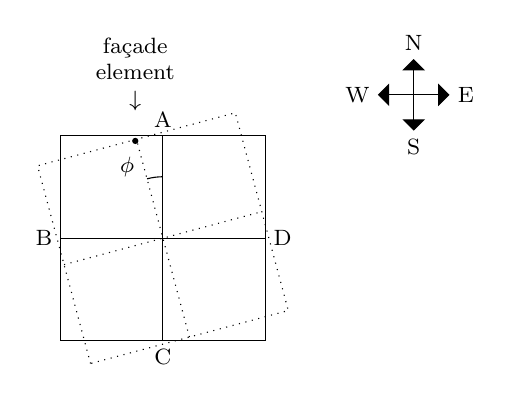
\begin{tikzpicture}[scale=1.3]
\footnotesize
\draw  (-1,-1) rectangle (1,1);
\draw  (0,-1) -- (0,1);
\draw  (-1,0) -- (1,0);
\draw [dotted,rotate around={15:(0,0)}] (-1,-1) rectangle (1,1);
\draw [dotted,rotate around={15:(0,0)}] (0,-1) -- (0,1);
\draw [dotted,rotate around={15:(0,0)}] (-1,0) -- (1,0);


\draw (-0.27,0.95) node[circle,fill,inner sep=0.8pt,align=center, label=below:]  (1) {};

\node [above, align=center] at (-0.27,0.95) {fa\c{c}ade \\ element \\ $\downarrow$ \\ };

\draw ([shift=(0:0cm)]0,0.6) arc (90:105:0.6cm);
\node [left] (nodela) at (-0.2,0.7) {$\phi$};

\draw (-1,-1) rectangle (1,1);
\node [left] at (-1,0.0) {B};
\node [right] at (1,0) {D};
\node [below] at (0,-1) {C};
\node [above] at (0,1) {A};


\begin{scope} [scale=0.7,shift={(3.5,2)}]
\coordinate (north) at (0,0.5);
\coordinate (east) at (0.5,0);
\coordinate (south) at (0,-0.5);
\coordinate (west) at (-0.5,0);

\draw [triangle 90-triangle 90] (north) -- (south);
\draw [triangle 90-triangle 90] (east) -- (west);
\node [above] (N) at (north) {N};
\node [right] (E) at (east) {E};
\node [below] (S) at (south) {S};
\node [left] (N) at (west) {W};
\end{scope}

\end{tikzpicture}

%\end{document}
	}
	\caption{Design situation}
	\label{tikz:design_situation}
\end{figure}






\subsection{Data under study}

\subsubsection{Wind speed data}
\begin{framed}
	To what extent will we mention that it matters how you discretize?
\end{framed}
For the probabilistic description of the $N$-yearly extreme wind speed, 'potential wind speed' parent data are used which are obtained from the KNMI-measurement station at Schiphol Airport. The potential wind speed data correspond to an hourly mean wind speed  at a reference height of $z_{ref}$ = 10 m and a standard terrain roughness of $z_{0,ref}$ = 0.03 m. The measurement period covers 64 years and the potential wind speeds are documented for every single hour. The accompanying incident wind-directions are documented for wind speed sections of $10^{\circ}$ which are combined to sections of $30^{\circ}$ (see Figure \ref{fig:incident_wind_directions}). 
A more detailed description of the wind speed data is provided in Meinen (2015).  


\subsubsection{Pressure coefficient data}\label{subsubsec:pressure_coefficient_data}
\begin{framed}
	To what extent will we mention that it matters how you discretize?
\end{framed}
For the description of the peak external pressure coefficients wind tunnel measurements are used which are obtained from the open-circuit atmospheric boundary layer wind tunnel of TNO with a full-scale terrain roughness $z_0=0.8$ m. The pressures are measured at taps placed at 172 locations on the building. In total two types of wind tunnel measurements are performed. The first type is called the 'long-run' experiment, where the incident flow is frontal only ($0^{\circ}\pm7.5^{\circ}$ for building orientation $\phi=0^{\circ}$), but of considerable long duration (approximately 175 hours in full scale). The second type is called the 'short-run' experiment, where the incident flow direction changed in sections of 15$^{\circ}$, but of shorter duration (approximately 30 minutes in full scale). The sections of $15^{\circ}$ are combined to sections of 30$^{\circ}$ (see Figure \ref{fig:incident_wind_directions2}). A more detailed description of the experimental materials, wind tunnel characteristics and executed measurements is provided in Meinen (2015).



\begin{figure}[H]
	\begin{minipage}[]{0.5\textwidth}
		%\documentclass[fleqn]{article}
%\usepackage{graphicx} % om PostScript plaatje in te lassen
%\usepackage{here}     % voor geforceerde plaatsing figuren
%\usepackage{amsmath}
%\textwidth=17.0cm
%\textheight=22.0cm
%\topmargin=-1cm
%\oddsidemargin=-0.3cm
%\evensidemargin=-0.3cm
%
%%packages
%\usepackage{amsmath}
%\usepackage{cite}
%\usepackage[toc,page]{appendix}
%\usepackage{fancyvrb}
%\usepackage{tikz}
%\usepackage{multicol}
%\usepackage{framed}
%\usepackage{pgfplots}
%\usepackage{fixltx2e}
%\usepackage{subfigure}
%\usepackage{lscape}
%\usepackage{enumitem}
%\usepackage{multirow}
%\usepackage{color}
%\renewcommand*\descriptionlabel[1]{\hspace\leftmargin$#1$}
%
%%tikz labraries
%\usetikzlibrary{matrix}
%\usetikzlibrary{decorations.pathreplacing}
%\usetikzlibrary{positioning}
%\usetikzlibrary{calc}
%\usetikzlibrary{shapes,arrows, chains}
%\usetikzlibrary{intersections}
%\usetikzlibrary{decorations.markings}
%\usetikzlibrary{calc,intersections}
%\usetikzlibrary{patterns}
%\usepackage{xcolor}
%
%%\usetikzlibrary{decorations.pathreplacing,bending}
%
%%extra instellingen
%\newlist{aims}{enumerate}{1}
%\setlist[aims,1]{
%  label={*},
%  leftmargin=*,
%  align=left,
%  labelsep=2mm,
%}
%
%\newlist{aims2}{enumerate}{1}
%\setlist[aims2,1]{
%  label={},
%  leftmargin=0pt,
%  align=left,
%  labelsep=4mm,
%}
%
%\newlist{aims3}{enumerate}{1}
%\setlist[aims3,1]{
%  label={-},
%  leftmargin=2cm,
%  align=left,
%  labelsep=0.4mm,
%}
%
%\makeatletter
%\def\mathcolor#1#{\@mathcolor{#1}}
%\def\@mathcolor#1#2#3{%
%  \protect\leavevmode
%  \begingroup
%    \color#1{#2}#3%
%  \endgroup
%}
%\makeatother
%
%
%% overige instellingen
%\makeatletter
%\newcommand\frontmatter{%
%    \cleardoublepage
%  \@mainmatterfalse
%  \pagenumbering{roman}}
%\newcommand\mainmatter{%
%    \cleardoublepage
%  \@mainmattertrue
%  \pagenumbering{arabic}}
%\newcommand\backmatter{%
%  \if@openright
%    \cleardoublepage
%  \else
%    \clearpage
%  \fi
% \@mainmatterfalse}
%\makeatother
%
%
%
%
%
%\begin{document}

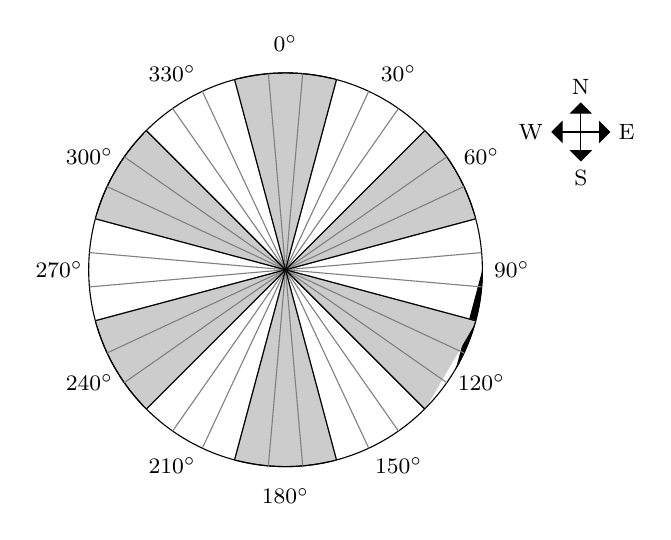
\begin{tikzpicture}[scale=2.5]
\footnotesize

\filldraw[fill=black!20, rotate=-15] (0,1) arc (90:120:1cm);
\draw[black!20, fill=black!20, rotate=-15] (0,0) -- ($(0,0)!1cm!(0,1)$) to ($(0,0)!1cm!(-0.37,0.65)$)  -- cycle;

\begin{scope}[rotate=60]
\filldraw[fill=black!20, rotate=-15] (0,1) arc (90:120:1cm);
\draw[black!20, fill=black!20, rotate=-15] (0,0) -- ($(0,0)!1cm!(0,1)$) to ($(0,0)!1cm!(-0.37,0.65)$)  -- cycle;
\end{scope}

\begin{scope}[rotate=120]
\filldraw[fill=black!20, rotate=-15] (0,1) arc (90:120:1cm);
\draw[black!20, fill=black!20, rotate=-15] (0,0) -- ($(0,0)!1cm!(0,1)$) to ($(0,0)!1cm!(-0.37,0.65)$)  -- cycle;
\end{scope}

\begin{scope}[rotate=180]
\filldraw[fill=black!20, rotate=-15] (0,1) arc (90:120:1cm);
\draw[black!20, fill=black!20, rotate=-15] (0,0) -- ($(0,0)!1cm!(0,1)$) to ($(0,0)!1cm!(-0.37,0.65)$)  -- cycle;
\end{scope}

\begin{scope}[rotate=240]
\filldraw[fill=black!20, black=-15] (0,1) arc (90:120:1cm);
\draw[black!20, fill=black!20, rotate=-15] (0,0) -- ($(0,0)!1cm!(0,1)$) to ($(0,0)!1cm!(-0.37,0.65)$)  -- cycle;
\end{scope}

\begin{scope}[rotate=300]
\filldraw[fill=black!20, rotate=-15] (0,1) arc (90:120:1cm);
\draw[black!20, fill=black!20, rotate=-15] (0,0) -- ($(0,0)!1cm!(0,1)$) to ($(0,0)!1cm!(-0.37,0.65)$)  -- cycle;
\end{scope}


\draw (0,0) circle (1cm);


\begin{scope}[rotate=90]
\foreach \k in {0, 30, 60, 90, 120, 150, 180,  210,240, 270, 300, 330}
{
\node at (-\k:1.15) {\k $^{\circ}$};
}
\end{scope}




\foreach \i in {5, 15, 25, 35, 45, 55, 65, 75, 85, 95, 105, 115, 125, 135, 145, 155, 165, 175}
{
\draw [gray, rotate=\i] (0,-1) -- (0,1);
}

\foreach \i in {15, 45, 75, 105, 135, 165}
{
\draw [black, rotate=\i] (0,-1) -- (0,1);
}



\begin{scope}[shift={(1.5,0.7)}, scale=0.15]
\coordinate (north) at (0,1);
\coordinate (south) at (0,-1);
\coordinate (east) at (1,0);
\coordinate (west) at (-1,0);
\draw [triangle 90-triangle 90] (north) -- (south);
\draw [triangle 90-triangle 90] (east) -- (west);
\node [above] (N) at (north) {N};
\node [right] (E) at (east) {E};
\node [below] (S) at (south) {S};
\node [left] (N) at (west) {W};
\end{scope}

\end{tikzpicture}

%\end{document}
		\caption{Discretized incident wind-directions for sections of 30$^{\circ}$ - wind speeds}
		\label{fig:incident_wind_directions}
	\end{minipage}
	\hspace{0.4cm}
	\begin{minipage}[]{0.5\textwidth}
		%\documentclass[fleqn]{report}
%\usepackage{graphicx} % om PostScript plaatje in te lassen
%\usepackage{here}     % voor geforceerde plaatsing figuren
%\usepackage{amsmath}
%\textwidth=17.0cm
%\textheight=22.0cm
%\topmargin=-1cm
%\oddsidemargin=-0.3cm
%\evensidemargin=-0.3cm
%
%%packages
%\usepackage{amsmath}
%\usepackage{cite}
%\usepackage[toc,page]{appendix}
%\usepackage{fancyvrb}
%\usepackage{tikz}
%\usepackage{multicol}
%\usepackage{framed}
%\usepackage{pgfplots}
%%\usepgfplotslibrary{fillbetween}
%\usepackage{fixltx2e}
%\usepackage{subfigure}
%\usepackage{lscape}
%\usepackage{enumitem}
%\usepackage{filecontents}
%\usetikzlibrary{decorations.pathmorphing}
%\usepackage{lmodern}
%\usepackage{pgfplotstable}
%
%\usetikzlibrary{arrows}
%%\usetikzlibrary{arrows.meta}
%
%
%
%\usetikzlibrary{decorations.pathreplacing,decorations.markings,snakes}
%
%%tikz labraries
%\usetikzlibrary{matrix}
%\usetikzlibrary{decorations.pathreplacing}
%\usetikzlibrary{positioning}
%\usetikzlibrary{calc}
%\usetikzlibrary{shapes,arrows, chains}
%\usetikzlibrary{patterns}
%
%\usetikzlibrary{intersections}
%\usetikzlibrary{decorations.markings}
%\usetikzlibrary{calc,intersections}
%%\usetikzlibrary{decorations.pathreplacing,bending}
%
%%extra instellingen
%\newlist{aims}{enumerate}{1}
%\setlist[aims,1]{
%  label={*},
%  leftmargin=*,
%  align=left,
%  labelsep=2mm,
%}
%
%\newlist{aims2}{enumerate}{1}
%\setlist[aims2,1]{
%  label={},
%  leftmargin=0pt,
%  align=left,
%  labelsep=4mm,
%}
%
%\newlist{aims3}{enumerate}{1}
%\setlist[aims3,1]{
%  label={-},
%  leftmargin=2cm,
%  align=left,
%  labelsep=0.4mm,
%}
%
%\usepackage{pgfplots}
%
%\begin{document}
%\begin{figure}
%\centering
%
%





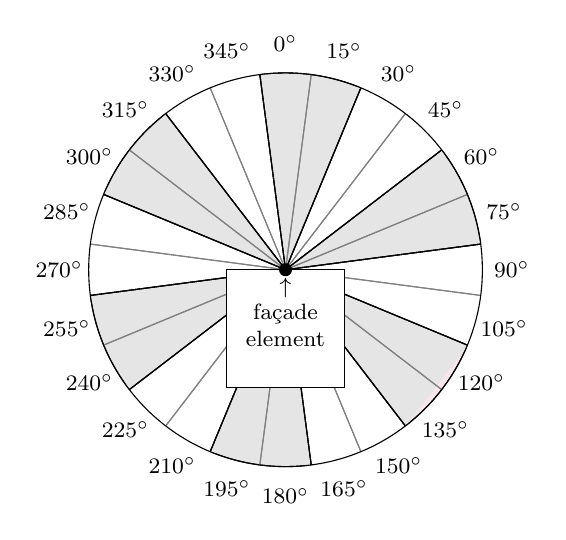
\begin{tikzpicture}[scale=2.5]

\footnotesize

\begin{scope}[rotate=-22.5]

\filldraw[fill=black!10] (0,1) arc (90:120:1cm);
\draw[black!10, fill=black!10] (0,0) -- ($(0,0)!1cm!(0,1)$) to ($(0,0)!1cm!(-0.37,0.65)$)  -- cycle;

\begin{scope}[rotate=60]
\filldraw[fill=black!10] (0,1) arc (90:120:1cm);
\draw[black!10, fill=black!10] (0,0) -- ($(0,0)!1cm!(0,1)$) to ($(0,0)!1cm!(-0.37,0.65)$)  -- cycle;
\end{scope}

\begin{scope}[rotate=120]
\filldraw[fill=black!10] (0,1) arc (90:120:1cm);
\draw[black!10, fill=black!10] (0,0) -- ($(0,0)!1cm!(0,1)$) to ($(0,0)!1cm!(-0.37,0.65)$)  -- cycle;
\end{scope}

\begin{scope}[rotate=180]
\filldraw[fill=black!10] (0,1) arc (90:120:1cm);
\draw[black!10, fill=black!10] (0,0) -- ($(0,0)!1cm!(0,1)$) to ($(0,0)!1cm!(-0.37,0.65)$)  -- cycle;
\end{scope}

\begin{scope}[rotate=240]
\filldraw[fill=purple!10] (0,1) arc (90:120:1cm);
\draw[black!10, fill=black!10] (0,0) -- ($(0,0)!1cm!(0,1)$) to ($(0,0)!1cm!(-0.37,0.65)$)  -- cycle;
\end{scope}

\begin{scope}[rotate=300]
\filldraw[fill=black!10] (0,1) arc (90:120:1cm);
\draw[black!10, fill=black!10] (0,0) -- ($(0,0)!1cm!(0,1)$) to ($(0,0)!1cm!(-0.37,0.65)$)  -- cycle;
\end{scope}
\end{scope}

\begin{scope}[rotate=7.5]
\foreach \i in {0, 15, 30, 45, 60, 75, 90, 105, 120, 135, 150, 165, 180, 195, 210, 225, 240, 255, 270, 285, 300, 315, 330, 345}
{
\draw [gray, rotate=\i] (0,-1) -- (0,1);
}
\foreach \i in {0, 30, 60, 90, 120, 150, 180, 210, 240, 270, 300, 330}
{
\draw [black, rotate=\i] (0,-1) -- (0,1);
}
\end{scope}

\draw (0,0) circle (1cm);


\begin{scope}[rotate=90]
\foreach \k in {0, 15, 30, 45, 60, 75, 90, 105, 120, 135, 150, 165, 180, 195, 210, 225, 240, 255, 270, 285, 300, 315, 330, 345}
{
\node at (-\k:1.15) {\k $^{\circ}$};
}
\end{scope}


\begin{scope}[scale=0.3]
\begin{scope}[shift={(0,-1)}]
\footnotesize
\draw [fill=white] (-1, -1) rectangle (1,1);
\draw [fill=black] (0, 1) circle (0.1);
\node [below, align=center] at (0,1) {$\uparrow$ \\ fa\c{c}ade \\ element};
\end{scope}
\end{scope}


\end{tikzpicture}

%\end{figure}
%
%\end{document}
		\caption{Discretized incident wind-directions for sections of 30$^{\circ}$ - pressure coefficients}
		\label{fig:incident_wind_directions2}
	\end{minipage}
\end{figure}




\subsection{Derivation probabilistic models}
First step is to obtain the probabilistic models for each of the parameters mentioned in PARAGRAPH.


\subsubsection{Structural resistance}
Step by step explanation on how the distribution function..

First step is to determine the design value of the load effects as 

Mayybe first we need to explain how the design value oft he structural resistance is obtained. That was missing in my previous paper. \\
\\
First step is to determine the design value of the structural resistance... Here we use




This limits to the data
\subsubsection{Probabilistic description of the extreme wind speeds}
\begin{framed}
Codification of wind load for structural design requires the estimation of the quantiles or return period values of the annual maximum wind speed. The wind speed of interest can be the hourly-mean wind speed [1] or the gust wind speed (ASCE-07). Given wind records, the tasks of extreme value analysis of wind speed for a single meteorological station are: the extraction of necessary number of samples of maximum wind speed from the wind records with/without an imposed threshold; the choice of probabilistic model (e.g., the selection of probability distribution type); and the extreme value analysis using the selected model and extracted data. The peak or maximum wind speed data can be extracted based on several criteria: maximum per specified time interval (e.g., per year), over a specified threshold, or the r-th largest values. The major advantage of using annual extreme values is the simplicity in data processing, although its use potentially reduces the amount of available wind data that can be considered for extreme analysis. The use of the r-th largest order statistics [2], and the data over a peak threshold can ameliorate the data scarcity, but the results could be sensitive to the size of r and the threshold selected. Moreover, if multiyear and multi-station data are considered, significant efforts are needed to process and inspect the data and to ensure that they are from independent events.

Extreme value analysis of the annual maximum wind speed at a site by using different probabilistic models was presented and debated (e.g., Refs. [3–7]). It seems that the Gumbel distribution is the most widely used probabilistic model for extreme value wind speed analysis [8–11]. This distribution has no upper bound, although use of a distribution without finite upper end point for extreme wind speed has been criticized on thermodynamic ground, but a justifiable finite upper end point is unclear. The distribution fitting methods used include the method of moments, the method of the maximum likelihood, the generalized least-squares, and the method of L-moments (MLM) [12]. The use of the generalised Pareto distribution and the generalized extreme value (GEV) distribution to maximum wind speeds has also been considered [4,13]. The application of generalised Pareto distribution is debated [4,5,7]. For the wind speed data from 235 meteorological stations in Canada, the at-site extreme value analysis results and the calculated values of the Akaike information criterion (AIC) [14] indicate that the Gumbel model for majority of stations outperforms the GEV distribution [15].
\end{framed}




According to paragraph \ref{subsubsec:windpseeds}, for each incident wind-direction the yearly extreme hourly mean wind speeds are obtained, resulting in 64 extremes for each incident wind-direction. Table \ref{table:tab:V_sample_statistics_max}                                                            column 2-5  provides the numerical summaries of the extremes, where $\hat{\mu}_v$ indicates the sample mean, $\hat{\text{V}}_v$ the sample variance and $\hat{\alpha}_v$  the sample skewness. The characteristics of the yearly extreme hourly mean wind speeds differ greatly for the distinct incident wind-directions. E.g. the sample mean $\hat{\mu}_v$ variates between 10.1 m/s for $\theta_i=120^{\circ}$ to 19.7 m/s for $\theta_i=240^{\circ}$. Thereby the highest mean wind speeds are found between $210^{\circ}\leq \theta_i\leq 270^{\circ}$, representing the winds coming from the South-West direction. The sample coefficient of variation $\hat{\text{V}}_v$ variates between 0.12   for $\theta_i=210^{\circ}$ and 0.18 for $\theta_i=0^{\circ}$. The sample skewness $\hat{\alpha}_v$ variates between 0.44  for $\theta_i=270^{\circ}$ and 1.56 for $\theta_i=120^{\circ}$. It is also observed that the parent wind coming from incident wind-direction $\theta_i$ is not uniformly distributed throughout the wind-rose; wind speeds coming from the South-West direction clearly have a higher probability of occurrence than the wind speeds coming from other directions. 


\begin{table}[H]                                                                                     
	\footnotesize
	\centering                                                                                            
	\caption{Numerical summaries and Gumbel model parameters of the yearly extreme hourly mean wind speeds as a function of the incident wind-direction $\theta_i$}
	\label{table:tab:V_sample_statistics_max}                                                             
	\begin{tabular}{|c|c|c|c|c|c|c|}                                                                    
		\hline
		&  \multicolumn{4}{|c|}{numerical summaries}             & \multicolumn{2}{|c|}{Gumbel model parameters} \\ \hline                                                                                              
		$\theta_i\pm15^{\circ}$ &	$\hat{\mu_v}$	&	$\hat{\text{V}}_v$	&	$\hat{\alpha}_v$	&	$p(\theta_i)$	&	$\alpha$	&	$u$	\\	\hline
		0$^{\circ}$	&	13.2	&	\textbf{0.18}	&	0.76	&	0.06	&	0.51	&	12.07	\\	\hline
		30$^{\circ}$	&	12.4	&	0.13	&	0.59	&	0.06	&	0.77	&	11.69	\\	\hline
		60$^{\circ}$	&	12.6	&	0.14	&	0.64	&	0.08	&	0.68	&	11.79	\\	\hline
		90$^{\circ}$	&	11.1	&	0.18	&	1.16	&	0.07	&	0.67	&	10.26	\\	\hline
		120$^{\circ}$	&	\textbf{10.1}	&	0.16	&	\textbf{1.56}	&	0.05	&	0.86	&	9.41	\\	\hline
		150$^{\circ}$	&	11.8	&	0.14	&	0.70	&	0.07	&	0.73	&	11.04	\\	\hline
		180$^{\circ}$	&	14.3	&	0.14	&	0.91	&	0.10	&	0.62	&	13.35	\\	\hline
		210$^{\circ}$	&	17.6	&	\textbf{0.12}	&	0.95	&	0.14	&	0.56	&	16.63	\\	\hline
		240$^{\circ}$	&	\textbf{19.7}	&	0.14	&	0.52	&	0.12	&	0.43	&	18.42	\\	\hline
		270$^{\circ}$	&	18.3	&	0.17	&	\textbf{0.44}	&	0.10	&	0.38	&	16.81	\\	\hline
		300$^{\circ}$	&	17.2	&	0.17	&	0.77	&	0.07	&	0.41	&	15.83	\\	\hline
		330$^{\circ}$	&	15.4	&	0.17	&	1.40	&	0.07	&	0.53	&	14.23	\\	\hline
	\end{tabular}
\end{table}

% illustration
\begin{figure}[H] 
	\centering    
	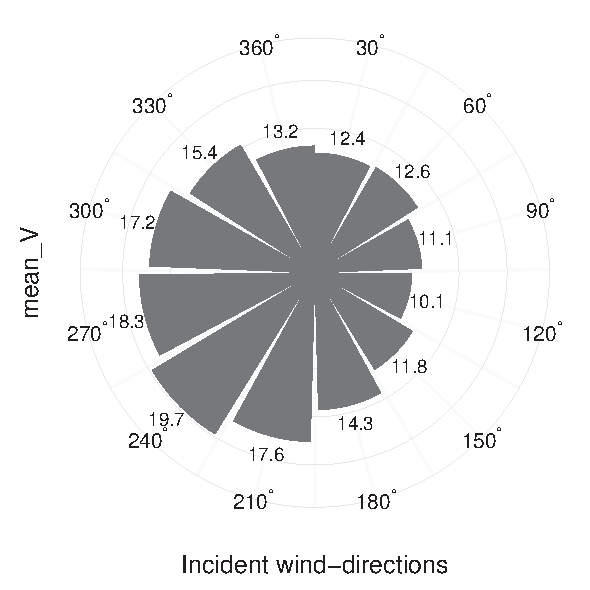
\includegraphics[width=0.4\textwidth]{images/Schiphol_mean_V_test.pdf}
	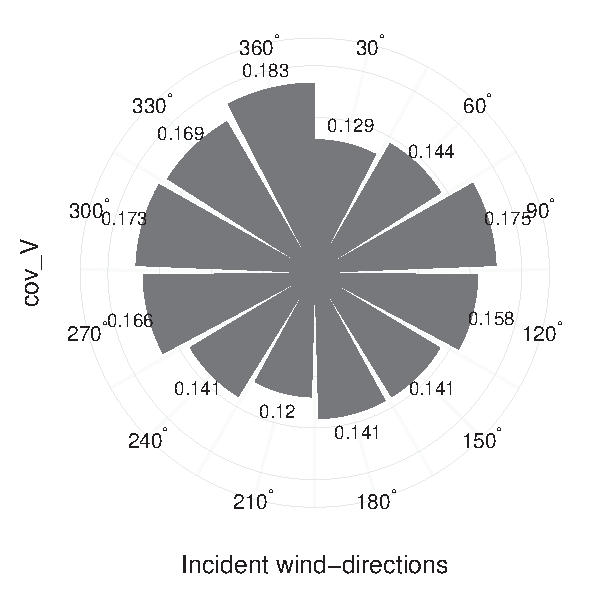
\includegraphics[width=0.4\textwidth]{images/Schiphol_cov_V_test.pdf}
	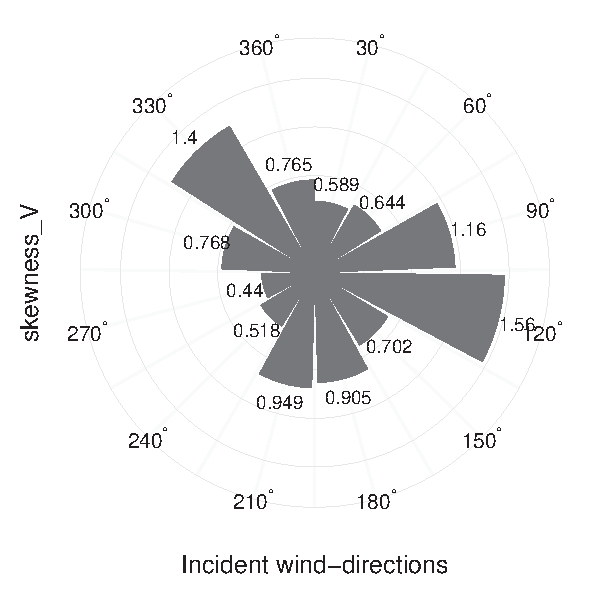
\includegraphics[width=0.4\textwidth]{images/Schiphol_skewness_V_test.pdf}
	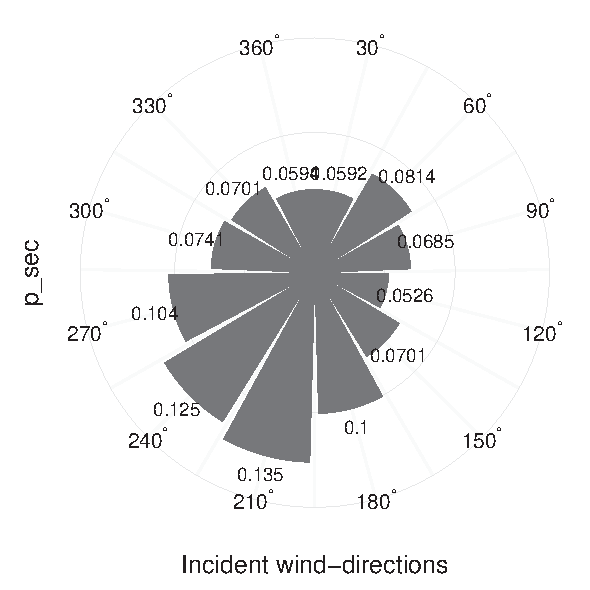
\includegraphics[width=0.4\textwidth]{images/Schiphol_p_sec_test.pdf}
	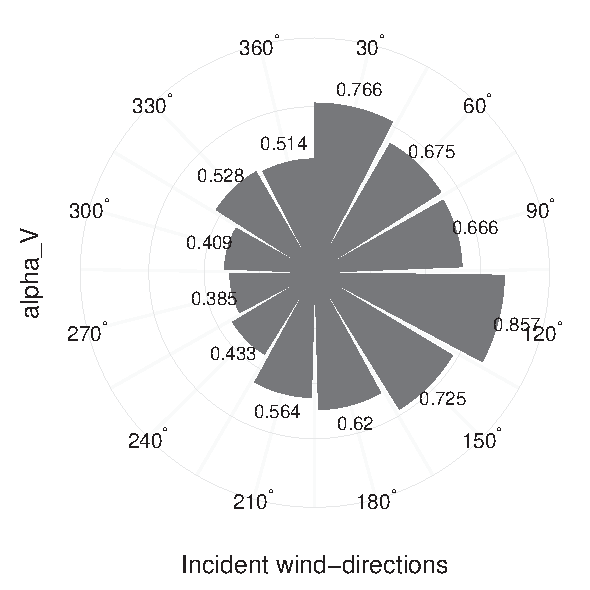
\includegraphics[width=0.4\textwidth]{images/Schiphol_alpha_V_test.pdf}
	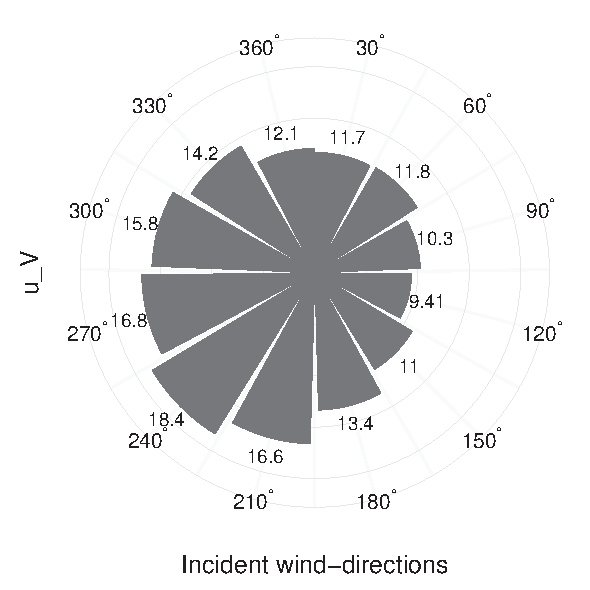
\includegraphics[width=0.4\textwidth]{images/Schiphol_u_V_test.pdf}
	\caption{Numerical summaries and Gumbel model parameters of the yearly extreme hourly mean wind speeds as a function of the incident wind-direction $\theta_i$}
	\label{fig:compass_summary_wind}
\end{figure}

\noindent
For each incident wind-direction the Gumbel distribution is fitted on the yearly extreme hourly mean wind speeds. The parameters of the Gumbel distribution are provided in table \ref{table:tab:V_sample_statistics_max} column 6-7.                                                       
Figure \ref{figure_V_240} and \ref{figure_V_270} show the model distribution functions together with the sample data for the governing incident wind-directions, plotted in the Gumbeldomain. 
It is observed that, towards the higher probability fractiles, the discrepancy between the sample data and the distribution function increases. 


\begin{figure}[H]
	\begin{minipage}[]{0.5\textwidth}
		\centering
		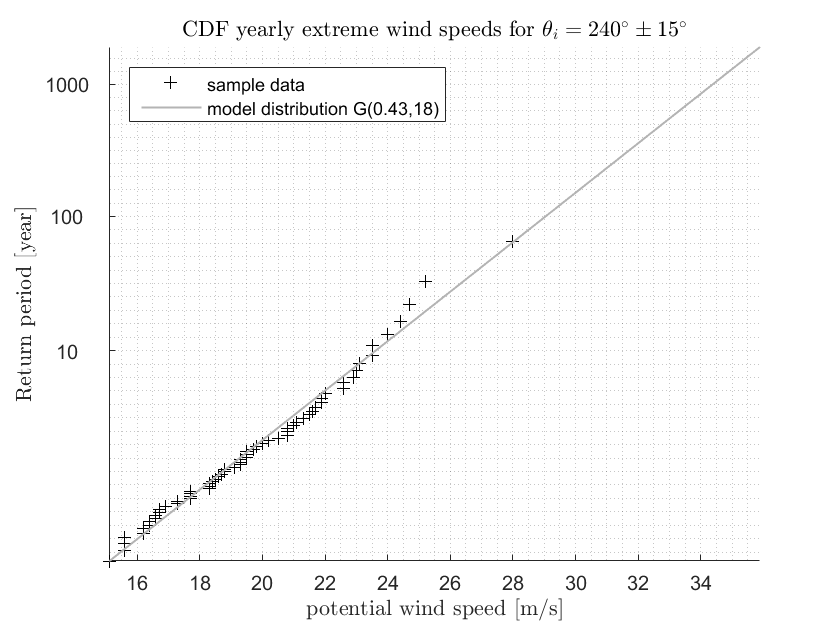
\includegraphics[scale=0.4]{images/CDF_yearly_extreme_windspeeds_G}
		\caption{Cumulative distribution  function (CDF) of the yearly extreme hourly mean wind speeds for $\theta_i=240^{\circ}\pm 15^{\circ}$}
		\label{figure_V_240}
	\end{minipage}
	\hspace{0.4cm}
	\begin{minipage}[]{0.5\textwidth}
		\centering
		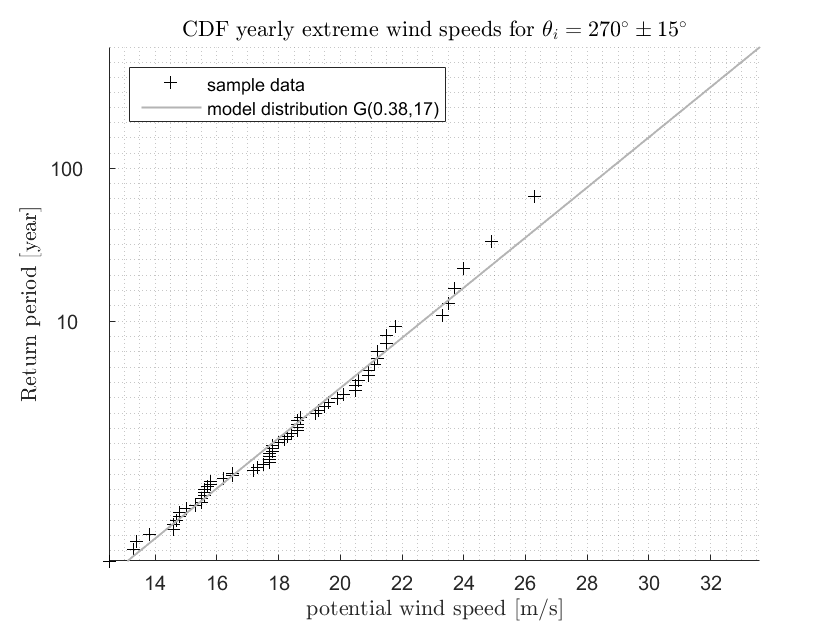
\includegraphics[scale=0.4]{images/CDF_yearly_extreme_windspeeds_G270}
		\caption{Cumulative distribution function (CDF) of the yearly extreme hourly mean wind speeds for $\theta_i=270^{\circ}\pm 15^{\circ}$}
		\label{figure_V_270}
	\end{minipage}
\end{figure}

\subsubsection{Probabilistic description of the hourly extreme pressure coefficients}
For the determination of the minimum required block-duration $t$ use is made of the 175 hour 'long run' wind tunnel data. In Meinen (2015) it was found that the value $t$ where the envelope autocorrelation function is equal to $R_{xx}(t)\leq0.2$ is approximately $t=10$ s. The block-duration chosen for further analysis is therefore $t=10$ s. \\
\\
Based on the 30 minutes 'short-run' wind-tunnel data for each incident wind-direction the the 10s-extreme peak external pressure coefficients are obtained, both for the maxima ($\hat{c}_{pe}$) and for the minima ($\check{c}_{pe}$), resulting in $2\cdot180$ extremes for each incident wind-direction. By analyzing the characteristics of the sample data it was observed that for the incident wind-directions
$\theta_i=7.5^{\circ}$, $\theta_i=37.5^{\circ}$ and $\theta_i=307.5^{\circ}$ and $\theta_i=337.5^{\circ}$ the maxima were governing, where for all other incident wind-directions the minima were governing. Table \ref{table:descriptive_statistics_C}                                                              provides the numerical summaries of the 10s-extreme peak external pressure coefficients for each incident wind-direction $\theta_i$ accordingly. In the table $\hat{\mu}_c$ indicates the sample mean, $\hat{\text{V}}_c$ indicates the unbiased sample coefficient of variation and $\hat{\alpha}_c$ the sample skewness. On average, the highest maxima are found for incident wind-direction $\theta_i=7.5^{\circ}$, of which the mean is equal to $\mu_{c}=1.1$. On average, the highest minima are found for incident wind-direction $\theta_i=277.5^{\circ}$, of which the mean is equal to $\mu_{c}=-1.3$. The coefficient of variation $\hat{\text{V}}_{c}$ variates between 0.12 for incident wind-direction $\theta_i=217.5^{\circ}$ and 0.36 for incident wind-direction $\theta=67.5^{\circ}$. The sample skewness $\hat{\alpha}_c$ variates between -1.65  for incident wind-direction $\theta=247.5^{\circ}$ and 0.16  for incident wind-direction $\theta=37.5^{\circ}$.  \\
\\
It is remarked that the highest extremes are found for incident wind-direction $\theta_i=67.5^{\circ}$ and not for incident wind-direction $\theta_i=277.5^{\circ}$. This is attributed to the fact that the coefficient of variation of incident wind-direction $\theta_i=67.5^{\circ}$ is larger than the coefficient of variation for incident wind-direction $\theta_i=277.5^{\circ}$. 



\begin{table}[H]                                                                                     
	\footnotesize
	\centering                                                                                            
	\caption{Numerical summaries and Gumbel model parameters of the 10s extreme peak external pressure coefficients as a function of the incident wind-direction $\theta_i$}
	\label{table:descriptive_statistics_C}                                                             
	\begin{tabular}{|c|c|c|c|c|c|c|}                                                                    
		\hline
		&               &\multicolumn{3}{|c|}{numerical summaries}  &\multicolumn{2}{|c|}{model parameters}             \\ \hline
		$\theta_i\pm15^{\circ}$	&	max/min	&	$\hat{\mu_c}$	&	$\hat{\text{V}}_c$ &	$\hat{\alpha}_c$	&	$\alpha$	&	$u$	\\	\hline
		7.5$^{\circ}$	&	max	&	\textbf{1.1}	&	0.13	&	-0.40	&	6.49	&	1.06	\\	\hline
		37.5$^{\circ}$	&	max	&	0.9	&	0.20	&	\textbf{0.16}	&	6.22	&	0.78	\\	\hline
		67.5$^{\circ}$	&	min	&	-1.0	&	\textbf{0.36}	&	0.06	&	2.83	&	-0.82	\\	\hline
		97.5$^{\circ}$	&	min	&	-1.2	&	0.24	&	-0.68	&	4.28	&	-1.05	\\	\hline
		127.5$^{\circ}$	&	min	&	-0.6	&	0.12	&	-0.43	&	16.92	&	-0.54	\\	\hline
		157.5$^{\circ}$	&	min	&	-0.6	&	0.12	&	-0.49	&	17.21	&	-0.52	\\	\hline
		187.5$^{\circ}$	&	min	&	-0.5	&	0.19	&	-0.89	&	11.97	&	-0.48	\\	\hline
		217.5$^{\circ}$	&	min	&	-0.5	&	\textbf{0.12}	&	-0.34	&	16.01	&	-0.50	\\	\hline
		247.5$^{\circ}$	&	min	&	-0.7	&	0.18	&	\textbf{-1.65}	&	11.29	&	-0.61	\\	\hline
		277.5$^{\circ}$	&	min	&	\textbf{-1.3}	&	0.21	&	-0.36	&	4.13	&	-1.15	\\	\hline
		307.5$^{\circ}$	&	max	&	0.6	&	0.24	&	0.14	&	7.8	&	0.53	\\	\hline
		337.5$^{\circ}$	&	max	&	1.1	&	0.15	&	0.11	&	6.73	&	0.98	\\	\hline
	\end{tabular}
\end{table}

\noindent
For each incident wind-direction the Gumbel distribution is fitted on the 10s-extreme peak external pressure coefficients. 
The parameters of the Gumbel distribution are provided in Table 
\ref{table:descriptive_statistics_C}                                                              column 6-7. Figure \ref{fig:C_maxima} and \ref{fig:C_minima} show respectively the model distributions of the 10s-maximum and 10s-minimum peak external pressure coefficients for the governing incident wind-directions, plotted in the Gumbeldomain. The sample data show a curved behaviour in the Gumbeldomain. As a consequence, in the higher probability fractiles, the Gumbel distributions (which show a straight line in the Gumbeldomain by definition) deviate significantly from the sample data. A similar behaviour is found for most other incident wind-directions. 

\begin{figure}[H]
	\begin{minipage}[]{0.5\textwidth}
		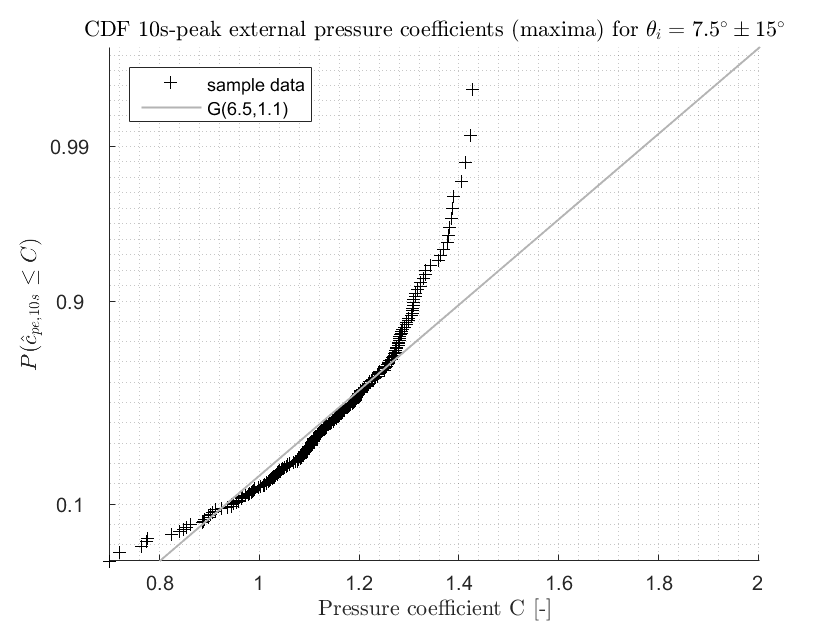
\includegraphics[scale=0.4]{images/CDF_10s_peak_external_pressure_coefficients_maxima_G}
		\caption{Cumulative distribution function (CDF) of the 10s-maximum peak external pressure coefficients for incident wind-direction $\theta_i=7.5^{\circ}\pm15^{\circ}$} \label{fig:C_maxima}
	\end{minipage}
	\hspace{0.4cm}
	\begin{minipage}[]{0.5\textwidth}
		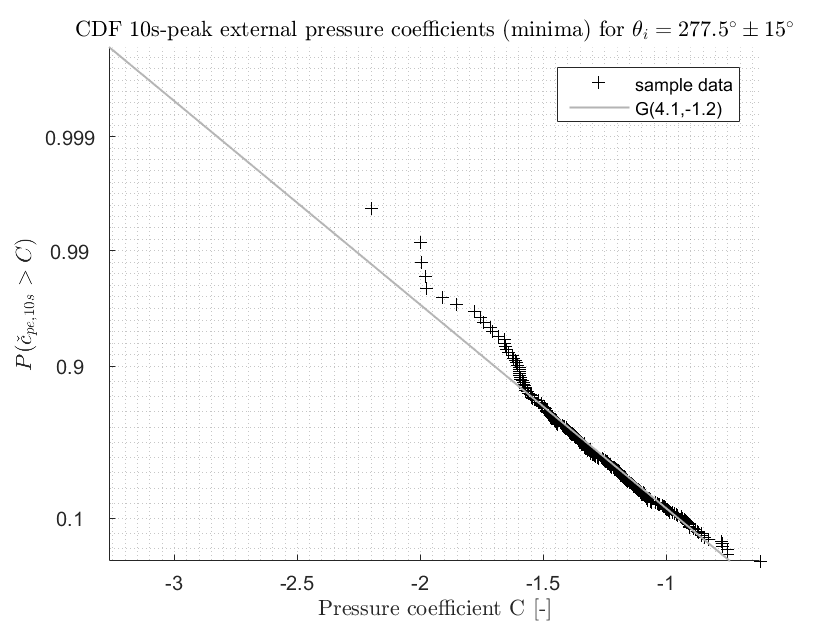
\includegraphics[scale=0.4]{images/CDF_10s_peak_external_pressure_coefficients_minima_G}
		\caption{Cumulative distribution function (CDF) of the 10s-minimum peak external pressure coefficients for incident wind-direction $\theta_i=277.5^{\circ}\pm15^{\circ}$} \label{fig:C_minima}
	\end{minipage}
\end{figure}



\subsubsection{Results reliability calculations}
For each building orientation $\phi$ the total failure probability of the fa\c{c}ade element is determined according to equations \ref{limit_state_function} to \ref{beta_total}. Figure \ref{fig:total_reliability_all_directiosn} shows  the resulting reliability indices $\beta_{total}$. The figure shows that the structural reliability is strongly dependent on the building orientation. Reliability indices are found between $\beta_{total}= 3.1$ for the governing building orientation $\phi=187.5^{\circ}$ and $\beta_{total}=4.6$ for the most advantageous building orientation $\phi=277.5^{\circ}$. It is remarked that the governing building orientation is that orientation where the  governing wind speeds (coming from incident wind-direction $\theta_i=240^{\circ}$) are combined with the governing peak external pressure coefficients (coming from incident wind-direction $\theta_i= 67.5^{\circ}$).\\
\\
Figure \ref{fig:direction_dependent_beta_values} shows the direction-dependent unconditional $\beta$-values for the governing building orientation $\phi=187.5^{\circ}$. Additionally the figure shows $\beta_{total}$ plotted as a horizontal black line. The direction-dependent unconditional $\beta$-values differ greatly for the incident wind-directions. Unconditional $\beta$-values are found between $\beta(\theta_i)=3.1$ for $\theta_i=240^{\circ}$ to $\beta(\theta_i)> 8$ for $\theta_i=30^{\circ}$. In terms of the failure probability, this differs several orders of magnitude. Consequentially, the total structural reliability is almost fully determined by incident wind-direction $\theta=240^{\circ}$ only;  the influence of all other incident wind-directions is negligibly small. A similar one-direction dominance is found for all other building orientations. In most cases the dominant incident wind-direction lies within $210^{\circ} \leq\theta_i \leq 270^{\circ}$, representing the wind speeds coming from the South-West direction.\\
\\
Table \ref{alpha-values} shows the averaged sensitivity factors ($\alpha$-values) for all incident wind-directions and all orientations of the building. The $\alpha$-values are highest for the hourly extreme wind speeds, with an average of $\alpha_{v_{hr,N}} = -0.83$. The $\alpha$-values are lowest for the structural resistance and the model uncertainty factor, with $\alpha_R=0.22$ and $\alpha_{\chi_{model}}=-0.20$ respectively. It is remarked that the observed $\alpha_R$-value of the structural resistance lies far from the chosen $\alpha_R=0.8$ in subsection \ref{sec:as}. 





\begin{figure}[H]
	\begin{minipage}[]{0.5\textwidth}
		\centering
		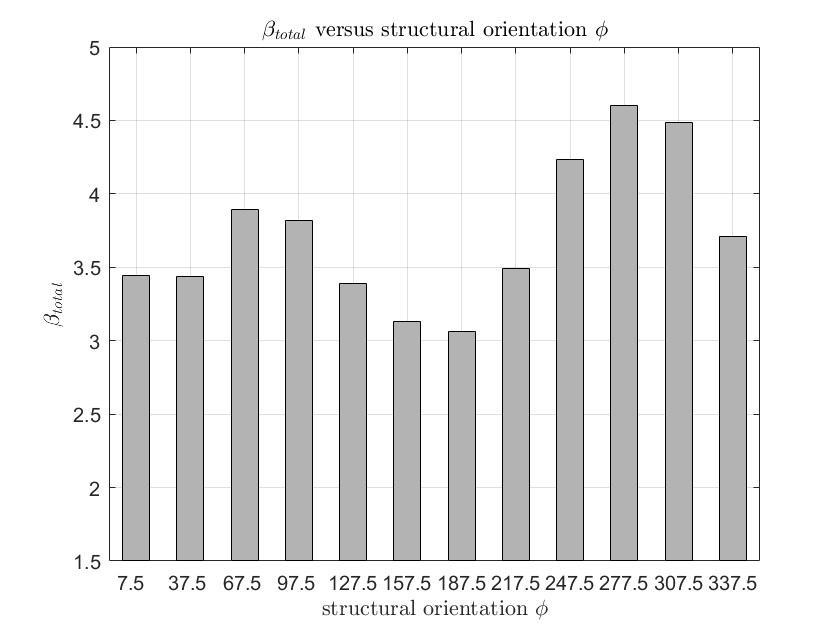
\includegraphics[scale=0.4]{images/beta_total_orientation_G}
		\caption{$\beta_{total}$-values versus building orientation $\phi$ \textcolor{white}{$\beta_{total}$-values versus building orientation $\phi$} \textcolor{white}{$\beta_{total}$-values versus building orientation $\phi$}}
		\label{fig:total_reliability_all_directiosn}
	\end{minipage}
	\hspace{0.4cm}
	\begin{minipage}[]{0.5\textwidth}
		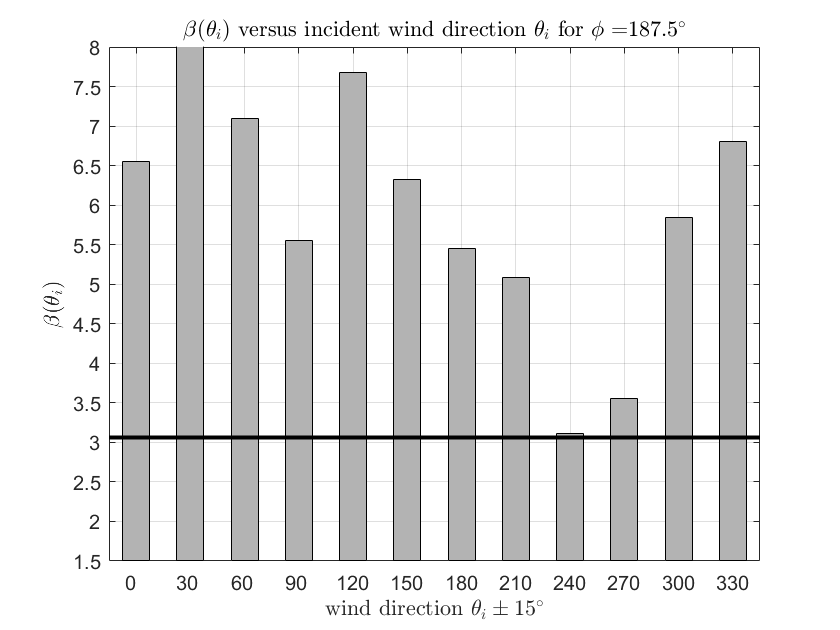
\includegraphics[scale=0.4]{images/unconditional_beta_values_G}
		\caption{Direction-dependent unconditional $\beta$-values versus incident wind-direction $\theta_i$, for building oriention $\phi=187.5^{\circ}$} \label{fig:direction_dependent_beta_values}
	\end{minipage}
\end{figure}

\begin{table}[htb!]
	\centering
	\caption{Averaged $\alpha$-values for all incident wind directions and all orientations of the building}
	\label{alpha-values}
	\begin{tabular}{|l|l|l|}
		\hline
		parameter              & $\mu$ & $\sigma$ \\ \hline
		$\alpha_R$    & 0.22 & 0.01  \\ \hline
		$\alpha_{v_{hr,N}}$             & -0.83 & 0.02  \\ \hline
		$\alpha_{\hat{c}_{pe,hr}}$      & -0.32 & 0.05  \\ \hline
		$\alpha_{c_r^2}$                & -0.33 & 0.01  \\ \hline
		$\alpha_{\chi_{model}}$         & -0.20 & 0.01  \\ \hline
	\end{tabular}
\end{table}

\section{Discussion}\label{discussion}
\textit{Discussion of case-study results}\\
The results show that, due to the wind-directionality effects, the  structural reliability of wind-loaded fa\c{c}ade elements is strongly dependent on the building-orientation, resulting in $\beta_{total}$ values between $3.1\leq\beta_{total}\leq4.6$. In case the wind-directionality effects would not have been taken into account, the outcome of the reliability analysis would be independent of the building orientation and furthermore lower. Especially for the non-governing building orientations this would result in too conservative estimations of the structural reliability. Accounting for wind-directionality effects in the assessment of fa\c{c}ade elements may therefore be extremely advantageous for the design. Similar conclusions have been drawn by Davenport (1983) and Simiu and Filliben (1981).  \\
\\
Furthermore it was found that the total failure probability was almost fully determined by the governing incident wind-directions only; the failure probabilities due to all other incident wind-directions were found to be negligibly small. These results provide arguments for the development of a more practical assessment procedure in the future, where the structural reliability of the fa\c{c}ade element is assessed on the basis of the governing incident wind-directions only. \\
\\
\textit{Discussion of assessment procedure}\\
Even though the results of the case study give good insight in the wind-directionality effects, there are still some remarks to be made concerning the assessment procedure as such. \\
\\
Due to the limited duration of both the wind speed and the wind-tunnel measurements,  the number of sample data available for distribution fitting is relatively small. This introduces large statistical uncertainties in the estimation of the model parameters, which has been shown by Simiu et al. (1978) and Rojiani and Wen (1980). For a better estimation of the structural reliability these statistical uncertainties need to be incorporated in the assessment procedure. \\
\\
Furthermore, for both the extreme wind speeds and the extreme pressure coefficients, the Gumbel fit showed discrepancies with the sample data in the higher probability fractiles. Especially in the case of the extreme pressure coefficients the Gumbel distribution results in a too conservative tail-behaviour. This was also remarked by Kasperski (2003).
In order to assess this discrepancy the distribution skewness is compared with the sample skewness. The sample skewness provides information on the tail behaviour of the random variable, as it is very sensitive for extreme deviations from the mean. In case of the extreme pressure coefficients the sample skewness was found to vary between $-1.65 \leq \hat{\alpha}_c \leq 0.16$. In case of the extreme wind speeds the sample skewness was found to vary between $0.44 \leq \hat{\alpha}_v \leq 1.56$. The  distribution skewness of the Gumbel distribution, however, is fixed to 1.14 for maxima and -1.14 for minima. In many cases this fixed distribution skewness lies far away from the observed sample skewness, explaining the poor fit in the tail.
A better agreement between the sample skewness and the distribution skewness could be obtained the application of a distribution function with a non-fixed distribution skewness, for example the three parameter lognormal distribution or the Weibull distribution. A second option could be the application of a distinct statistical method for the modeling of the extremes, for example the peak-over-threshold method.\\
\\
The structural resistance $R$ was modeled as a lognormally distributed stochastic random variable with a coefficient of variation of $\text{V}_R=0.1$. The design-resistance $R_d$ was assumed to correspond to the EN1990 Level I probability of non-exceedance, with associated sensitivity factor $\alpha_R=0.8$. This chosen sensitivity factor lies far away from the observed sensitivity factor  $\alpha_R=0.22$, which is to be explained by the large uncertainties in the wind-loading part.
For the further development of the assessment procedure it is  recommended to use realistic resistance models for different failure mechanisms and different material types. In this way less assumptions need to be made concerning the design-values of the resistance parameters, as these are fixed according to their characteristic values and partial factors. \\
\\
Finally it is recommended to do further research in the probabilistic modeling of the roughness factor $c_r$ and the model uncertainty factor $\chi_{model}$, which are currently modeled on the basis of approximate literature only. 

\section{Conclusion}\label{conclusions}
In this research an assessment procedure is developed which is able to determine the structural reliability of wind-loaded fa\c{c}ade elements in terms of the failure probability. The assessment procedure accounts for the uncertainties in the extreme wind speeds, the extreme pressure coefficients, the factor correcting for terrain roughness, the structural resistance and the uncertainties in the wind-load model as such. For the modeling of the extreme wind speeds and the extreme pressure coefficients location-specific wind speed and pressure coefficient measurements are being used. The assessment procedure accounts explicitly for the effects of wind-directionality. \\
\\
In order to show its potential, the assessment procedure is applied on a case-study. It is found that the structural reliability of wind-loaded fa\c{c}ade elements is strongly dependent on the building orientation, differing in failure probabilities of several orders of magnitude. Additionally it is found that the failure probability is almost fully determined by the governing incident wind-directions only; the contribution of all other incident wind-directions were found to be negligibly small. \\
\\
For the future developments of the assessment procedure it is recommended to further investigate appropriate statistical methods for the modeling of the extreme wind speeds and the extreme pressure coefficients, to additionally account for the sampling uncertainties in the modeling of the extreme wind speeds and the extreme pressure coefficients, to use realistic resistance models for different failure mechanisms and different material types and, finally, to further investigate the probabilistic description of the roughness factor and the model uncertainty factor.


\nocite{*}
\bibliographystyle{plain}
\bibliography{References}




%
%
%\end{document}


%\documentclass[fleqn]{article}
%\usepackage{graphicx} 
%\usepackage{here}    
%\usepackage{amsmath}
%\textwidth=15.0cm
%\textheight=22.0cm
%\topmargin=-1cm
%\oddsidemargin=-0.3cm
%\evensidemargin=-0.3cm
%
%
%%packages
%\usepackage{amsmath}
%\usepackage{cite}
%\usepackage[toc,page]{appendix}
%\usepackage{fancyvrb}
%\usepackage{tikz}
%\usepackage{multicol}
%\usepackage{framed}
%\usepackage{pgfplots}
%\usepackage{fixltx2e}
%\usepackage{subfigure}
%\usepackage{lscape}
%\usepackage{enumitem}
%\usepackage{multirow}
%\usepackage{color}
%\usepackage{xcolor}
%\usepackage{comment}
%\usepackage{changes}
%\renewcommand*\descriptionlabel[1]{\hspace\leftmargin$#1$}
%
%%tikz labraries
%\usetikzlibrary{matrix}
%\usetikzlibrary{decorations.pathreplacing}
%\usetikzlibrary{positioning}
%\usetikzlibrary{calc}
%\usetikzlibrary{shapes,arrows, chains}
%\usetikzlibrary{intersections}
%\usetikzlibrary{decorations.markings}
%\usetikzlibrary{calc,intersections}
%\usetikzlibrary{patterns}
%
%
%\makeatletter
%\def\mathcolor#1#{\@mathcolor{#1}}
%\def\@mathcolor#1#2#3{%
%  \protect\leavevmode
%  \begingroup
%    \color#1{#2}#3%
%  \endgroup
%}
%\makeatother
%
%%##### DEFINE YOUR NAME #########################
%\definechangesauthor[color=blue,name={Arpad Rozsas}]{AR}
%\definechangesauthor[color=red,name={Nadieh Meinen}]{NEM}
%%###########################################
%
%\begin{document}

\section{Discussion}\label{discussion}
\textit{Discussion of case-study results}\\
The results show that, due to the wind-directionality effects, the  structural reliability of wind-loaded fa\c{c}ade elements is strongly dependent on the building-orientation, resulting in $\beta_{total}$ values between $3.1\leq\beta_{total}\leq4.6$. In case the wind-directionality effects would not have been taken into account, the outcome of the reliability analysis would be independent of the building orientation and furthermore lower. Especially for the non-governing building orientations this would result in too conservative estimations of the structural reliability. Accounting for wind-directionality effects in the assessment of fa\c{c}ade elements may therefore be extremely advantageous for the design. Similar conclusions have been drawn by Davenport (1983) and Simiu and Filliben (1981).  \\
\\
Furthermore it was found that the total failure probability was almost fully determined by the governing incident wind-directions only; the failure probabilities due to all other incident wind-directions were found to be negligibly small. These results provide arguments for the development of a more practical assessment procedure in the future, where the structural reliability of the fa\c{c}ade element is assessed on the basis of the governing incident wind-directions only. \\
\\
\textit{Discussion of assessment procedure}\\
Even though the results of the case study give good insight in the wind-directionality effects, there are still some remarks to be made concerning the assessment procedure as such. \\
\\
Due to the limited duration of both the wind speed and the wind-tunnel measurements,  the number of sample data available for distribution fitting is relatively small. This introduces large statistical uncertainties in the estimation of the model parameters, which has been shown by Simiu et al. (1978) and Rojiani and Wen (1980). For a better estimation of the structural reliability these statistical uncertainties need to be incorporated in the assessment procedure. \\
\\
Furthermore, for both the extreme wind speeds and the extreme pressure coefficients, the Gumbel fit showed discrepancies with the sample data in the higher probability fractiles. Especially in the case of the extreme pressure coefficients the Gumbel distribution results in a too conservative tail-behaviour. This was also remarked by Kasperski (2003).
In order to assess this discrepancy the distribution skewness is compared with the sample skewness. The sample skewness provides information on the tail behaviour of the random variable, as it is very sensitive for extreme deviations from the mean. In case of the extreme pressure coefficients the sample skewness was found to vary between $-1.65 \leq \hat{\alpha}_c \leq 0.16$. In case of the extreme wind speeds the sample skewness was found to vary between $0.44 \leq \hat{\alpha}_v \leq 1.56$. The  distribution skewness of the Gumbel distribution, however, is fixed to 1.14 for maxima and -1.14 for minima. In many cases this fixed distribution skewness lies far away from the observed sample skewness, explaining the poor fit in the tail.
A better agreement between the sample skewness and the distribution skewness could be obtained the application of a distribution function with a non-fixed distribution skewness, for example the three parameter lognormal distribution or the Weibull distribution. A second option could be the application of a distinct statistical method for the modeling of the extremes, for example the peak-over-threshold method.\\
\\
The structural resistance $R$ was modeled as a lognormally distributed stochastic random variable with a coefficient of variation of $\text{V}_R=0.1$. The design-resistance $R_d$ was assumed to correspond to the EN1990 Level I probability of non-exceedance, with associated sensitivity factor $\alpha_R=0.8$. This chosen sensitivity factor lies far away from the observed sensitivity factor  $\alpha_R=0.22$, which is to be explained by the large uncertainties in the wind-loading part.
For the further development of the assessment procedure it is  recommended to use realistic resistance models for different failure mechanisms and different material types. In this way less assumptions need to be made concerning the design-values of the resistance parameters, as these are fixed according to their characteristic values and partial factors. \\
\\
Finally it is recommended to do further research in the probabilistic modeling of the roughness factor $c_r$ and the model uncertainty factor $\chi_{model}$, which are currently modeled on the basis of approximate literature only. 

\section{Conclusion}\label{conclusions}
In this research an assessment procedure is developed which is able to determine the structural reliability of wind-loaded fa\c{c}ade elements in terms of the failure probability. The assessment procedure accounts for the uncertainties in the extreme wind speeds, the extreme pressure coefficients, the factor correcting for terrain roughness, the structural resistance and the uncertainties in the wind-load model as such. For the modeling of the extreme wind speeds and the extreme pressure coefficients location-specific wind speed and pressure coefficient measurements are being used. The assessment procedure accounts explicitly for the effects of wind-directionality. \\
\\
In order to show its potential, the assessment procedure is applied on a case-study. It is found that the structural reliability of wind-loaded fa\c{c}ade elements is strongly dependent on the building orientation, differing in failure probabilities of several orders of magnitude. Additionally it is found that the failure probability is almost fully determined by the governing incident wind-directions only; the contribution of all other incident wind-directions were found to be negligibly small. \\
\\
For the future developments of the assessment procedure it is recommended to further investigate appropriate statistical methods for the modeling of the extreme wind speeds and the extreme pressure coefficients, to additionally account for the sampling uncertainties in the modeling of the extreme wind speeds and the extreme pressure coefficients, to use realistic resistance models for different failure mechanisms and different material types and, finally, to further investigate the probabilistic description of the roughness factor and the model uncertainty factor.


\nocite{*}
\bibliographystyle{plain}
\bibliography{References}



%
%
%
%\end{document}
%

%\documentclass[fleqn]{article}
%\usepackage{graphicx} 
%\usepackage{here}    
%\usepackage{amsmath}
%\textwidth=15.0cm
%\textheight=22.0cm
%\topmargin=-1cm
%\oddsidemargin=-0.3cm
%\evensidemargin=-0.3cm
%
%
%%packages
%\usepackage{amsmath}
%\usepackage{cite}
%\usepackage[toc,page]{appendix}
%\usepackage{fancyvrb}
%\usepackage{tikz}
%\usepackage{multicol}
%\usepackage{framed}
%\usepackage{pgfplots}
%\usepackage{fixltx2e}
%\usepackage{subfigure}
%\usepackage{lscape}
%\usepackage{enumitem}
%\usepackage{multirow}
%\usepackage{color}
%\usepackage{xcolor}
%\usepackage{comment}
%\usepackage{changes}
%\renewcommand*\descriptionlabel[1]{\hspace\leftmargin$#1$}
%
%%tikz labraries
%\usetikzlibrary{matrix}
%\usetikzlibrary{decorations.pathreplacing}
%\usetikzlibrary{positioning}
%\usetikzlibrary{calc}
%\usetikzlibrary{shapes,arrows, chains}
%\usetikzlibrary{intersections}
%\usetikzlibrary{decorations.markings}
%\usetikzlibrary{calc,intersections}
%\usetikzlibrary{patterns}
%
%
%\makeatletter
%\def\mathcolor#1#{\@mathcolor{#1}}
%\def\@mathcolor#1#2#3{%
%  \protect\leavevmode
%  \begingroup
%    \color#1{#2}#3%
%  \endgroup
%}
%\makeatother
%
%%##### DEFINE YOUR NAME #########################
%\definechangesauthor[color=blue,name={Arpad Rozsas}]{AR}
%\definechangesauthor[color=red,name={Nadieh Meinen}]{NEM}
%%###########################################
%
%\begin{document}

\section{Conclusion}\label{conclusions}
In this research an assessment procedure is developed which is able to determine the structural reliability of wind-loaded fa\c{c}ade elements in terms of the failure probability. The assessment procedure accounts for the uncertainties in the extreme wind speeds, the extreme pressure coefficients, the factor correcting for terrain roughness, the structural resistance and the uncertainties in the wind-load model as such. For the modeling of the extreme wind speeds and the extreme pressure coefficients location-specific wind speed and pressure coefficient measurements are being used. The assessment procedure accounts explicitly for the effects of wind-directionality. \\
\\
In order to show its potential, the assessment procedure is applied on a case-study. It is found that the structural reliability of wind-loaded fa\c{c}ade elements is strongly dependent on the building orientation, differing in failure probabilities of several orders of magnitude. Additionally it is found that the failure probability is almost fully determined by the governing incident wind-directions only; the contribution of all other incident wind-directions were found to be negligibly small. \\
\\
For the future developments of the assessment procedure it is recommended to further investigate appropriate statistical methods for the modeling of the extreme wind speeds and the extreme pressure coefficients, to additionally account for the sampling uncertainties in the modeling of the extreme wind speeds and the extreme pressure coefficients, to use realistic resistance models for different failure mechanisms and different material types and, finally, to further investigate the probabilistic description of the roughness factor and the model uncertainty factor.








%\end{document}



\section{Left-over material, to be considered at the final stage}

\begin{framed}
\paragraph{Other tings not yet mentioned}
\begin{itemize}
\item The influence of discretization on the results.
\item Paper of Effect of human error on the reliability of roof panel under uplift wind pressure
\end{itemize}
\end{framed}

\begin{framed}
\added[id=NEM]{Some other comparisons}\\
For an overview of some of these methods for extreme wind speeds see \cite{Palutikof_1999}. For an overview of method for the modeling of extreme pressure coefficients see for example \cite{Peng201411}. \\
\\
Ying and Pandey \cite{Ying_2005} provide a comparative assessment where they apply POT, MIS Standard-Gumbel and MG methods to common wind speed data sets and studied the differences in quantile estimates. Perrin \textit{et. all} \cite{Perrin_2006} compared the use of the Weibull-method with classical EV methods, and found that the "design wind speeds were several meters per second, increasing with increasing return period". \added[]{needs verification} It is remarked that, for reasons of simplicity, in codification purposes mostly the Gumbel distribution is applied. \\
\\
In the case of extreme wind speeds, also extensions to the classical methods exist, such as the Method of Independent Storms \cite{Cookbook, Harris_1999}. 
and extensions to these methods, such as the method of r-largest extremes \footnote{general reference to this}\cite{Twan_1988}.\\ 
\\
Given a time-series of the extreme wind speeds, two approaches have been proposed in the literature for estimating design wind loads. The first approach uses the time series of the extreme wind speeds to fit the Gumbel distribution (the common approach). The second approach uses the time series of the square of the wind speeds to fit the Gumbel distribution \cite[297]{Cook_1985}  \cite[254 and 256]{Naess_date}\added[id=NEM]{needs checking} \cite{Harris_1996}. The arguments for the latter rest on the assumption that the parent population fron which the extreme speeds are extracted is appropriately modeled by a distribution that is, approximately, of the Rayleigh type, of which the rate of convergence of the asymptotic Gumbel distribution of epochal maxima would be faster if the maxima consisted of dynamic pressures than if they consisted of wind speeds \cite[297]{Cook_1985} . Consequentially, the application of the first approach rather than the latter results in more conservative design loads \cite[297]{Cook_1985}. \\
Simiu \textit{et.al.} \cite{Simiu_2001} however investigated this assumption and state that "there is no convincing support that the Gumbel distribution should be used as a model for extreme dynamic pressures".  
\end{framed}

\begin{framed}
Alternative titles: 
\begin{itemize}
\item Reliability-based importance assessment of the elements in the probabilistic wind load model 
\item On the determination of the structural reliability of wind-loaded structural elements
\item The effects of uncertainty propagation in the probabilistic wind load model on the structural reliability of wind loaded structural members. 
\item The effect of uncertainty propagation in the probabilistic assessment of wind-loaded structural members. 
\item Uncertainty propagation analysis of the main components of the stochastic wind load model for local wind loads.
\item Reliability-based uncertainty propagation analysis of the main components of the probabilistic wind load model for structural members. 
\end{itemize}
In statistics, propagation of uncertainty (or propagation of error) is the effect of variables' uncertainties on the structural reliability
\end{framed}


\begin{framed}
\added[id=NEM]{Shorter version regarding the DWLC}\\
For the modeling of extreme wind loads the principles of the Davenport Wind Loading Chain (DWLC) are widely accepted\cite{Davenport_2002}. The DWLC recognizes that the wind loading is built up out of several components or links,  combined together into a chain (see Figure \ref{fig:wind_loading_chain}). It states that the wind load  
on a particular building or structure is determined by the combined effects of the local wind climate, which is determined by the large-scale weather systems; the local wind exposure, which is determined by the terrain roughness and topography; the aerodynamic characteristics of the building shape; and the potential for load increases due to possible wind-induced resonant vibrations. The last link in the DWLC recognizes that clear criteria must be in place for judging the acceptability of the predicted loads and responses for both ultimate limit states and serviceability limit states. 
The quantification of each component is a function of the incident wind direction.
\end{framed}


\begin{framed}
\textbf{To problem statement or to review:}

Although some studies investigated one of these shortcomings, to our knowledge no paper has provided a comprehensive study before where all three are addressed. For example some recent studies did account for the uncertainties in all links jointly, e.g. for the purpose of partial factor calibration Hansen [?] and Sedlacek [ref]. However, modeling choices and their effect on structural reliability were not investigated. In a super amazing, pioneering study Meinen investigated the influence of some modeling choices on the reliability level of a structural component. The results showed that NUMBERS [ref]. This paper is the extension of that study.
\end{framed}

\nocite{*}
\bibliographystyle{plain}
\bibliography{References}

\end{document}